\documentclass[11pt]{article}
\usepackage[T1]{fontenc}
\usepackage{lmodern}
\usepackage[margin=1in]{geometry}
\usepackage{amsmath,amssymb,amsthm,mathtools}
\usepackage{booktabs,enumitem,microtype,needspace}
\usepackage{tikz}
\usetikzlibrary{arrows.meta,positioning,calc,fit}
\usepackage{xcolor}
\definecolor{linkblue}{RGB}{28,70,105}
\usepackage[colorlinks=true,linkcolor=linkblue,citecolor=linkblue,urlcolor=linkblue]{hyperref}
\hypersetup{pdftitle={Exact Uniform Sampling of Contingency Tables with Arbitrary Margins},pdfauthor={OpenAI}}
\ifdefined\pdfinfoomitdate\pdfinfoomitdate=1\fi
\ifdefined\pdftrailerid\pdftrailerid{}\fi
\ifdefined\pdfsuppressptexinfo\pdfsuppressptexinfo=15\fi
\newtheorem{theorem}{Theorem}[section]
\newtheorem{lemma}[theorem]{Lemma}
\newtheorem{proposition}[theorem]{Proposition}
\newtheorem{corollary}[theorem]{Corollary}
\theoremstyle{definition}
\newtheorem{definition}[theorem]{Definition}
\theoremstyle{remark}
\newtheorem{remark}[theorem]{Remark}
\newcommand{\R}{\mathbb{R}}
\newcommand{\Z}{\mathbb{Z}}
\newcommand{\N}{\mathbb{N}}
\newcommand{\E}{\mathbb{E}}
\newcommand{\Pp}{\mathbb{P}}
\newcommand{\one}{\mathbf{1}}
\newcommand{\eps}{\varepsilon}
\newcommand{\norm}[1]{\lVert#1\rVert}
\newcommand{\abs}[1]{\lvert#1\rvert}
\DeclareMathOperator{\Var}{Var}
\DeclareMathOperator{\TV}{TV}
\DeclareMathOperator{\diag}{diag}
\DeclareMathOperator{\vol}{vol}
\DeclareMathOperator{\supp}{supp}
\setlist[itemize]{topsep=4pt,itemsep=2pt,parsep=0pt}
\setlist[enumerate]{topsep=4pt,itemsep=3pt,parsep=0pt}
\numberwithin{equation}{section}
\emergencystretch=1em

\title{Exact Uniform Sampling of Contingency Tables\\with Arbitrary Margins}
\author{OpenAI}
\date{September 24, 2026}
\begin{document}
\maketitle
\begin{abstract}
We give an exact uniform sampler for nonnegative integer contingency tables
with arbitrary prescribed margins. It terminates almost surely and has expected
bit complexity polynomial in both dimensions and the binary length of the
margins. No positivity, balance, sparsity, or fixed-dimension assumption is
required.
\end{abstract}
\section{Introduction}\label{sec:introduction}

For nonnegative integer vectors $r=(r_1,\ldots,r_m)$ and
$c=(c_1,\ldots,c_n)$ with common total $N$, write
\[
 \Omega(r,c)=\left\{X\in\Z_{\ge0}^{m\times n}:
       \sum_jX_{ij}=r_i,\quad \sum_iX_{ij}=c_j\right\}.
\]
The uniform distribution on this finite set gives every table equal mass.
We study sampling when both dimensions vary and the margins are encoded
in binary. In particular, a polynomial bound in the numeric total $N$
would not, in general, give a polynomial bound in the input length.
There are no cell bounds or forbidden positions: every nonnegative integer
matrix with the prescribed margins is allowed. For probability laws on a
finite set, we use the convention
$\TV(\mu,\nu)=\tfrac12\sum_x|\mu(x)-\nu(x)|$.

\begin{theorem}\label{thm:main}
For arbitrary nonnegative integer margins of equal total, the following
algorithms exist in the model of unbiased random bits and bit operations.
\begin{enumerate}[label=\textup{(\roman*)}]
 \item Given an integer $k\ge1$, a bounded-time algorithm outputs a table
 in $\Omega(r,c)$ whose law is within $2^{-k}$ in total variation of the
 uniform law. Its running time is polynomial in
 $m,n,\log(N+1),k$.
 \item An algorithm outputs an exactly uniform table in $\Omega(r,c)$,
 terminates almost surely, and has expected running time polynomial in
 $m,n,\log(N+1)$.
\end{enumerate}
The polynomials are uniform over all margin vectors. No positivity,
sparsity, balance, or fixed-dimension hypothesis is imposed.
\end{theorem}

For a rational tolerance $0<\eps<1$ encoded by a binary numerator and
denominator, integer comparisons compute
$k=\lceil\log_2(1/\eps)\rceil$ in time polynomial in that encoding length.
Thereafter part~\textup{(i)} has accuracy dependence polynomial in
$\log(1/\eps)$.
The algorithms below are explicit, although their exponents are deliberately
large. Part~\textup{(ii)} concerns expected time: an exceptionally rare
branch performs exhaustive computation.

\paragraph{Counting and sampling fixed-margin arrays.}
Contingency tables are a basic family of integer arrays with linear
constraints. Their enumeration and exact and approximate generation are
treated, for example, by Diaconis and Gangolli~\cite{DiaconisGangolli1995}.
The algorithmic question involves more than producing one feasible table:
the law must give all feasible tables nearly or exactly the same mass,
even when their number and the coordinate ranges are exponentially large
in the margin bit length.

For two rows, Dyer and Greenhill~\cite{DyerGreenhill2000} give polynomial-time
approximate counting and sampling. Their heat-bath chain has mixing time
at most $n(n-1)\log(N/\eps)/2$ in the author version's Theorem~4.1.
Dependence on $\log N$ rather than $N$ makes this a polynomial bound in
the binary input length.
Kijima and Matsui~\cite[Theorems~3.1 and~5.1]{KM2003} give exact uniform
sampling for two rows by monotone coupling from the past, after sorting
the columns. Their expected $O(n^3\ln N)$ bound is stated for pseudocode
using uniform real draws. These results allow arbitrary two-row margin
sizes after deleting zero margins.

The fixed-row case extends beyond two rows. Cryan and
Dyer~\cite{CD2003} combine dynamic programming with volume estimation for
approximate counting and sampling. Dyer~\cite[Section~3]{Dyer2003} gives a
dynamic-programming rejection sampler that is exactly uniform, analyzed
in arithmetic operations. Cryan, Dyer, Goldberg,
Jerrum, and Martin~\cite{CDGJM2006} prove rapid mixing of the
$2\times2$ heat-bath chain for every fixed number of rows.
The polynomial bounds in these results depend on that fixed row count;
they do not give a bound polynomial jointly in both dimensions.

DeSalvo and Zhao~\cite[Theorem~2.3 and Remarks~2.4--2.5]{DZ2016} give a
general exact divide-and-conquer construction using $O(mn\log M)$ expected
random bits, where $M$ is the largest margin. In the cited arXiv version,
their polynomial total-runtime conclusion is conditional on efficient
evaluation of the parity-restricted counting quantities in Conjecture~2.6;
the bit-time bounds in Theorem~\ref{thm:main} are unconditional.

Another line of work uses the geometry of the transportation polytope
when margins are large. Dyer, Kannan, and Mount~\cite{DKM1997} develop
scaled coordinates, softened constraints, lattice walks, and rounding
comparisons for dense tables. Morris~\cite{Morris2002} improves the dense
sampling bounds through expanded polytopes and rounding. These methods
are close antecedents of the dense completion routine below. Our use of
that routine is conditional: a padding construction makes every
completion problem dense, while a separate chain handles all cells
incident to small margins.

For sparse margins, Arman, Gao, and Wormald~\cite[Theorem~1 and
Remark~2]{AGW2021} give exact uniform generation under $5\Delta^4<N$,
where $\Delta$ is the largest margin, in expected $O(N)$ time with
unit-cost arithmetic on integers of magnitude $O(N)$. The condition is
a genuine restriction, although within this family it also bounds $N$
polynomially in the dimensions. Their 2021 introduction surveys fixed-row,
dense, and sparse algorithms and reports that no polynomial-time
approximately uniform sampler for arbitrary margins was then known.
Theorem~\ref{thm:main} removes those margin and dimension restrictions
and includes all random bits and integer arithmetic in its cost.

\paragraph{Approximation and exact correction.}
Exactness and bounded running time are separate issues. Our approximate
algorithm has a deterministic polynomial work bound for each accuracy
request. The final exact correction uses the residual-mixture construction
of G\"obel, Liu, Manurangsi, and Pappik~\cite[Section~3.1, Algorithm~1 and
Theorem~6]{GLMP2024}. That construction combines a sufficiently accurate
sampler with a rare exhaustive draw from the remaining probability mass.
Its application here requires an additional property: the actual
implemented output law can be tabulated in time with an exponential
input-size factor but only polynomial dependence on the accuracy bits.
We prove that property and give the dyadic implementation explicitly.
Thus the exact algorithm has polynomial expected bit cost, not a
polynomial bound on every execution.

\paragraph{Proof strategy.}
Only cells incident to a margin below a polynomial threshold are explicit
coordinates of the auxiliary chain. The remaining cells form a complete
rectangle. We pad this rectangle so every conditional completion problem
has large margins. Each explicit cell has two bounded integer values,
one for its row and one for its column. Besides states where these values
agree, called transversals, we allow a positive unit discrepancy at one
cell and a negative unit discrepancy at another.

The target law on these small states assigns weight equal to the number
of padded completions. Sampling a state from that law and then a uniform
completion makes all state/completion pairs equally likely. Accept only
a transversal whose large completion entries are all at least the
padding. Subtracting it then gives a uniform original table conditional
on acceptance.
Section~\ref{sec:graph} constructs a repair map for the defect states and
uses it to bound their weight and the probability of successful unpadding.
The bounded sampler never evaluates completion counts: an ideal transition
uses a uniform completion draw to test a proposed move.

To prove that this chain mixes in polynomial time, we expose the small-cell
values of a transversal in a fixed order. After fixing a prefix, we compare
the averages of any real function on the state graph over the two fibers
that assign adjacent values to the next cell. The comparison comes from
quadratic forms indexed by pairs of unit removals.
Section~\ref{sec:signatures} proves that these forms have at most
one positive eigenvalue and that the property survives summing out a
balanced pair. A weighted telescoping calculation then bounds the energy
of a signed flow between neighboring conditional fibers.
Section~\ref{sec:transport} combines this bound with conditional-variance
decomposition and repair to obtain a Poincar\'e inequality for the
completion-count law. This supplies the small chain's mixing bound.

Section~\ref{sec:dense} implements the completion draws approximately on
a finite scaled grid, using rational arithmetic and dyadic random choices.
A continuous log-concave density serves only as an analytic tool for the
rejection and conductance bounds. Large coordinate ranges appear in
finite sums in the proof but are never enumerated in an ordinary run.
Section~\ref{sec:algorithms} couples each implemented completion draw to
its ideal counterpart and bounds the number of sampling and unpadding
attempts, giving the bounded almost-uniform algorithm. For exactness,
it also shows how to tabulate that algorithm's actual finite law,
including its stopping rules and fallbacks. This exhaustive computation
is performed only on the rare correction branch.

\section{The binary model and the padded graph}\label{sec:graph}

This section separates bounded small coordinates from a complete rectangle
of large coordinates. Its repair map controls the mass of defect states;
padding then gives a uniform lower bound on the chance of recovering an
original table from a stationary state and its completion.

We count bit operations and use independent unbiased random bits.
All margins are nonnegative integers given in binary, with common total
$N$.  Accuracy is specified by an integer $k\ge1$, meaning error at most
$2^{-k}$.
An empty dimension forces $N=0$ and gives a unique empty table.
If $N=0$, or if one dimension is one, the unique table can likewise be
returned directly.  In all remaining constructions the dimensions are
positive, and we use
\begin{equation}\label{eq:parameters}
\begin{gathered}
 d=10+(m+1)(n+1),\qquad L=d^{12},\qquad U=d^{20},\\
 C=N+dL+U+2,\qquad b=d+\lceil\log_2(C+2)\rceil.
\end{gathered}
\end{equation}
Here $d$ is a dimension allowance, $L$ the padding, $U$ the small-margin
threshold, $C$ a coordinate cap, and $b$ a bit-size allowance.
Thus $d\ge14$, $mn<d$, $U<C$, and
$b=O(d+\log(N+1))$.  Polynomial bounds in $d,b,k$ have the required
binary-input dependence.  A fixed feasible table is obtained greedily:
choose a row and column of positive remaining margins, place the minimum
of those two margins in their cell, and subtract it from both margins.
Each placement exhausts a row or column.  This uses at most $m+n-1$
positive placements and polynomial bit work, including initialization of
the output.  We fix index order for this construction and all later ties.

\subsection{Small states and large completions}

Put $I=\{i:r_i\ge U\}$ and $J=\{j:c_j\ge U\}$.
The \emph{large slots} are the cells in the complete rectangle
$\mathcal B=I\times J$; the remaining cells form the set $\mathcal S$ of
\emph{small slots}.  Set $B_s=C$ on $\mathcal B$ and $B_s=U$ on
$\mathcal S$.  Associate to each slot two coordinates
$x_s,y_s\in\{0,\ldots,B_s\}$, and put $q_s=B_s-y_s$.
Here $x$ is the row viewpoint and $q$ is the column viewpoint.
A slot is \emph{balanced} when $x_s=q_s$, equivalently
$x_s+y_s=B_s$.
The balanced representation of a value $a\in\{0,\ldots,B_s\}$ is
$(x_s,y_s)=(a,B_s-a)$; both $x_s$ and $q_s$ then equal $a$.

A graph state retains only the coordinates on $\mathcal S$.
Its allowed pattern is either a \emph{transversal}, with all slots
balanced, or a \emph{defect}, with distinct slots $t,s$ satisfying
\[
 x_t=q_t+1,\qquad x_s=q_s-1,
 \qquad x_v=q_v\quad(v\notin\{s,t\}).
\]
We call $t$ positive and $s$ negative.  Both patterns have total doubled
occupancy $\sum_{s\in\mathcal S}(x_s+y_s)=U|\mathcal S|$.
Define the original residual margins by
\[
 R_i^0(X)=r_i-\sum_{j:(i,j)\in\mathcal S}x_{ij},\qquad
 P_j^0(X)=c_j-\sum_{i:(i,j)\in\mathcal S}q_{ij}.
\]
Their totals agree because $\sum_{s\in\mathcal S}(x_s-q_s)=0$.
Let $k_i$ and $\ell_j$ be the numbers of large slots in row $i$ and
column $j$.  A state is \emph{feasible} when all residuals are nonnegative
and $R_i^0=0$ if $k_i=0$, $P_j^0=0$ if $\ell_j=0$.
Its padded residuals and enlarged full margins are
\begin{align*}
 R_i(X)&=R_i^0(X)+k_iL,& P_j(X)&=P_j^0(X)+\ell_jL,\\
 \bar r_i&=r_i+k_iL,&\bar c_j&=c_j+\ell_jL.
\end{align*}
Write $\mathcal F_X$ for the set of nonnegative integer tables on
$\mathcal B$ with margins $R_i(X),P_j(X)$, and set
$f(X)=|\mathcal F_X|$.  On infeasible states set $f(X)=0$.
The complete rectangle admits a greedy completion whenever these
residual tests hold.  If $\mathcal B$ is empty the only completion is
the empty table, so feasible states have weight one.

Every completion has total at most $N+|\mathcal B|L<C$, and every
nonempty block margin is at least $L$.  In particular the formal large
capacity $C$ excludes no completion: its doubled coordinates can be
taken as $x_s=A_s,y_s=C-A_s$ for $A\in\mathcal F_X$.
The bounded sampler will draw completions of this block without
enumerating its large coordinate ranges.  One-row or one-column blocks have a
unique completion and need no random draw.

Let $\mathcal X$ be the feasible states, $\mathcal T\subseteq\mathcal X$
the transversals, and
\begin{equation}\label{eq:graph-masses}
 Z_0=\sum_{X\in\mathcal T}f(X),\qquad
 \Lambda=\sum_{X\in\mathcal X}f(X),\qquad
 \pi(X)=\frac{f(X)}{\Lambda}.
\end{equation}
An original feasible table gives a transversal and a completion by
retaining its small entries and adding $L$ to each large entry.
The small entries respect their capacity because every small cell has
an incident original margin below $U$.  This construction also gives a
specified starting transversal, using the greedy original table.

\subsection{Repairs and graph edges}

For a defect with negative slot $s=(i,j)$ and positive slot
$t=(i',j')$, put $v=(i',j)$.  With $e_w$ denoting a small-slot unit
vector, define its repair $\mathcal R(X)$ by
\begin{equation}\label{eq:repair-map}
 x'=x-e_t+\one_{\{v\in\mathcal S\}}e_v,
 \qquad q'=x',\qquad y'=U\one-q'.
\end{equation}
The term involving $e_v$ is omitted if $v$ is large.
The undirected graph on $\mathcal X$ contains all pairs that differ by
lowering one doubled small coordinate by one and raising another by
one, and also every pair $\{X,\mathcal R(X)\}$ with $X$ a defect.
Repeated edges are counted only once.  Its unnormalized energy is
\begin{equation}\label{eq:graph-energy}
 E(H)=\sum_{\{X,Y\}\text{ an edge}}
 \min\{f(X),f(Y)\}(H(X)-H(Y))^2.
\end{equation}

\begin{lemma}[Repair and preservation of prefixes]\label{lem:repair}
The repair is a feasible transversal.  For each fixed ordered pair
$(s,t)$ it is injective on small states and extends to an injection
\[
 (X,A)\longmapsto
 \begin{cases}
 (\mathcal R(X),A),&v\in\mathcal S,\\
 (\mathcal R(X),A+e_v),&v\in\mathcal B
 \end{cases}
 \quad(A\in\mathcal F_X).
\]
Thus $f(X)\le f(\mathcal R(X))$.
Order small slots by row and then by column.  If $t$ follows $s$, the
repair leaves every slot preceding $s$ unchanged.  When additionally
$x_s=l-1,q_s=l$, its repaired value at $s$ is $l$ if $i'=i$ and $l-1$
otherwise.
\end{lemma}
\begin{proof}
The defect relation is $q=x-e_t+e_s$, and $x_t\ge1$.
If $v$ is small, the changes to $x$ lie in row $i'$, with zero total;
the changes to $q$ are $q'-q=e_v-e_s$, in column $j$, also with zero
total.  Hence all residual margins are unchanged.
The new common entries are nonnegative.  Their row totals are the old
$x$ row totals and their column totals are the old $q$ column totals.
At each small slot, one of these totals is bounded by an original
margin strictly below $U$, proving the capacity constraint.
If $j'=j$, then $v=t$ and the two changes to $x$ cancel; the reset of
$q$ is confined to that column.  If $i'=i$, then $v=s$: the transfer
increments the negative slot, decrements the positive slot, and leaves
$q$ unchanged.  These include both possible coincidences.

If $v$ is large, it differs from $s,t$, and
$x'=x-e_t$, $q'=q-e_s$.  These vectors remain nonnegative and within
capacity, since $x_t\ge1$ and $q_s=x_s+1\ge1$.
Only the residuals of row $i'$ and column $j$ increase, each by one.
Both lines meet the large block.  Adding one to completion entry $v$
therefore gives a valid target completion.  Its entries remain below
$C$ by the total bound already proved.

For fixed $s,t$, the repaired vector recovers
$x=x'+e_t-\one_{\{v\in\mathcal S\}}e_v$, followed by
$q=x-e_t+e_s$ and $y=U\one-q$.  In the large-receiver case subtract
$e_v$ from the target completion; otherwise retain it.  These inverses
on the image prove both injections.

Finally, $t>s$ implies either $i'=i,j'>j$, in which case $v=s$, or
$i'>i$, in which case every small receiver $v$ follows $s$.
Only $s,t,v$ can change, proving prefix preservation and the claimed
special value.
\end{proof}

For later use, fix a balanced prefix $\sigma$ before $s$, and let
$z_-,z_+$ be the total transversal weights extending it with special
values $x_s=l-1,l$, respectively.  Let $c_{st,l}^{\sigma}$ be the total
weight of defects extending that prefix with negative $s$ satisfying
$x_s=l-1,q_s=l$ and positive $t>s$.  Lemma~\ref{lem:repair} maps this
entire class injectively, with completions, into one fixed child.  Hence
\begin{equation}\label{eq:conditional-repair}
 c_{st,l}^{\sigma}\le
 \begin{cases}z_+,&i'=i,\\z_-,&i'\ne i,\end{cases}
 \qquad\text{and in particular}\qquad
 c_{st,l}^{\sigma}\le\max\{z_-,z_+\}.
\end{equation}
Figure~\ref{fig:repair} illustrates the large-receiver case.
\begin{figure}[tb]
\centering
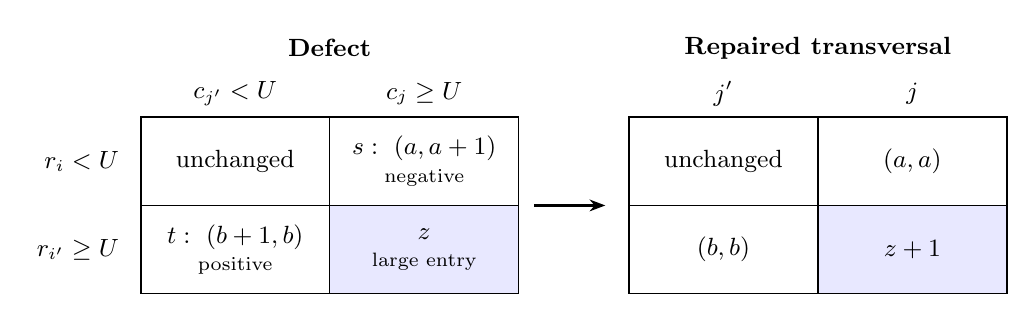
\begin{tikzpicture}[x=1cm,y=1cm,font=\small,
 cell/.style={minimum width=2.4cm,minimum height=1.12cm,inner sep=1pt},
 every path/.style={line width=.55pt}]
 \begin{scope}
  \fill[blue!9] (2.4,-2.24) rectangle (4.8,-1.12);
  \draw (0,0) rectangle (4.8,-2.24);
  \draw (2.4,0)--(2.4,-2.24);
  \draw (0,-1.12)--(4.8,-1.12);
  \node at (2.4,.88) {\textbf{Defect}};
  \node at (1.2,.3) {$c_{j'}<U$};
  \node at (3.6,.3) {$c_j\ge U$};
  \node[anchor=east] at (-.15,-.56) {$r_i<U$};
  \node[anchor=east] at (-.15,-1.68) {$r_{i'}\ge U$};
  \node[cell] at (1.2,-.56) {unchanged};
  \node[cell,align=center] at (3.6,-.56) {$s:\ (a,a+1)$\\[-1pt]\scriptsize negative};
  \node[cell,align=center] at (1.2,-1.68) {$t:\ (b+1,b)$\\[-1pt]\scriptsize positive};
  \node[cell,align=center] at (3.6,-1.68) {$z$\\[-1pt]\scriptsize large entry};
 \end{scope}
 \draw[-{Stealth[length=2mm]},thick] (5.0,-1.12)--(5.9,-1.12);
 \begin{scope}[xshift=6.2cm]
  \fill[blue!9] (2.4,-2.24) rectangle (4.8,-1.12);
  \draw (0,0) rectangle (4.8,-2.24);
  \draw (2.4,0)--(2.4,-2.24);
  \draw (0,-1.12)--(4.8,-1.12);
  \node at (2.4,.88) {\textbf{Repaired transversal}};
  \node at (1.2,.3) {$j'$};
  \node at (3.6,.3) {$j$};
  \node[cell] at (1.2,-.56) {unchanged};
  \node[cell] at (3.6,-.56) {$(a,a)$};
  \node[cell] at (1.2,-1.68) {$(b,b)$};
  \node[cell] at (3.6,-1.68) {$z+1$};
 \end{scope}
\end{tikzpicture}
\caption{The repair when the receiving cell $(i',j)$ is large.
Small cells display $(x,q)$, and the shaded cell displays a completion
entry. Decreasing $x_t$ and matching the viewpoints increases the
residual row margin at $i'$ and column margin at $j$ by one; adding
one to $z$ gives an injective map of completions.
The other cells remain unchanged.}
\label{fig:repair}
\end{figure}


There are fewer than $4d^2$ ordered unit exchanges.  A defect has one
designated repair; a transversal has at most $d^2$ inverse repairs,
one for each ordered defect type.  Thus the degree is at most
$5d^2+1$.  Neighbors can be listed with polynomial bit work using
\eqref{eq:repair-map} and its inverse, testing the boxes, patterns and
residuals, and removing duplicates.  No completion count is needed.
On a repair edge the weight in \eqref{eq:graph-energy} equals the
source defect's weight.

\subsection{Stationary mass and unpadding}

The repair bounds defect mass by transversal mass. To recover an original
table from a padded completion, we also need to control the probability
that a large entry is smaller than the padding. The following estimate
applies to unrestricted tables with any prescribed margins.

\begin{lemma}[Small entries]\label{lem:small-entry}
Consider the uniform law on all nonnegative integer tables with prescribed
margins, with at most $m$ rows and $n$ columns and no entry restrictions.
If both margins incident to a cell are at least $a\ge4d$, then, for every
integer $t$ with $0<t\le a/2$,
\[
 \Pp\{\text{the cell's entry is less than }t\}\le\frac{4td^3}{a}.
\]
\end{lemma}
\begin{proof}
Let the marked cell be $(i,j)$ and its entry be $h<t$.
The other entries in its row have sum at least $a/2$, as do the other
entries in its column.  Unless this event is empty, choose deterministically
$j'\ne j$ and $i'\ne i$ whose donor entries are both at least $a/(2d)$.
Such choices exist because each line has fewer than $d$ entries.  If there
is only one row or column, the event is empty instead.
For every $v=1,\ldots,\lfloor a/(2d)\rfloor$, subtract $v$ from the
entries $(i,j')$ and $(i',j)$ and add $v$ at $(i,j)$ and $(i',j')$.
The resulting table is nonnegative with the same margins.  Given this
table and the labels $(i',j',h)$, its marked entry determines $v$, and
reversing the four changes recovers the source.  There are at most $td^2$
possible labels for each output.  Since
$\lfloor a/(2d)\rfloor\ge a/(4d)$, double counting these moves gives
the asserted bound.  No upper entry bound is imposed in this argument.
\end{proof}

\begin{proposition}[Stationary mass and unpadding]\label{prop:stationary-success}
The masses satisfy
\begin{equation}\label{eq:stationary-mass-bounds}
 0<Z_0\le\Lambda\le(1+d^2)Z_0,
 \qquad \pi_{\min}\ge(C+1)^{-2d}.
\end{equation}
Draw $X$ with law $\pi$ and then a uniform $A\in\mathcal F_X$.
Declare success if $X$ is a transversal and every large entry of $A$
is at least $L$.  Subtracting $L$ from these entries gives a uniform
original table conditional on success, and
\begin{equation}\label{eq:unpadding-success}
 \Pp\{\text{success}\}\ge\frac{1}{2(1+d^2)}.
\end{equation}
\end{proposition}
\begin{proof}
For each of at most $|\mathcal S|(|\mathcal S|-1)\le d^2$ defect types,
the joint injection in Lemma~\ref{lem:repair} bounds its total weight
by $Z_0$.  This proves the upper bound on $\Lambda$; the other mass
inequalities follow from inclusion and the greedy starting table.
There are $\Lambda$ joint objects $(X,A)$, each specified by
$2|\mathcal S|+|\mathcal B|\le2mn<2d$ integer coordinates in $[0,C]$.
Thus $\Lambda\le(C+1)^{2d}$, and the positive integer weights $f(X)$
give the minimum-mass bound.

Consider all unrestricted tables with the enlarged margins
$\bar r,\bar c$, and call their number $F$.  Every transversal and
completion gives one such table, so $Z_0\le F$.
Each large cell has both enlarged margins at least $U$.
Lemma~\ref{lem:small-entry} and a union bound show that the proportion
of these enlarged tables with some large entry below $L$ is at most
\[
 |\mathcal B|\frac{4Ld^3}{U}\le\frac{4Ld^4}{U}
 =\frac4{d^4}<\frac12.
\]
Here $L\le U/2$ and $U\ge4d$; an empty block has no bad cells.
Every enlarged table passing this test can be unpadded to an original
table.  Conversely, padding every original table gives exactly one
passing table and a feasible transversal with its completion.
Consequently the successful pairs are in bijection with
$\Omega(r,c)$ and number at least $F/2\ge Z_0/2$.
Under the stated joint law every pair has probability
$(f(X)/\Lambda)(1/f(X))=1/\Lambda$, proving conditional uniformity
and \eqref{eq:unpadding-success}.
\end{proof}

If there are no small slots, $\mathcal X$ has one state and all graph
energies vanish; the completion and unpadding step still applies.
If there is no large block, the completion step is deterministic.
These conventions will also be used for the Markov chains below.

\section{Quadratic signatures and balanced summation}
\label{sec:signatures}

The transport construction uses quadratic forms with at most one positive
eigenvalue. We prove the required property for integer coordinates and then
show that it survives summation over balanced slots. Integer coordinates
allow two units to be removed at the same location, so the diagonal entries
and the endpoints of the summation require explicit treatment. Large
capacities occur only in finite mathematical sums in this section; the
algorithm will not enumerate those sums.
The one-positive-eigenvalue viewpoint is central to the theory of
Lorentzian polynomials developed by Br\"and\'en and Huh~\cite{BH2020}.
Here the needed closure is a discrete balanced-pair summation, established
by the laminar decomposition and telescoping calculation below.

\begin{definition}[Softened weights]\label{def:soft-weight}
Let $\mathcal B$ and $\mathcal S$ be the large and small slots from
Section~\ref{sec:graph}, and put
\[
 T=\sum_s B_s,\qquad
 \mathcal Q=\prod_s\{0,\ldots,B_s\}^2.
\]
For a full coordinate vector $\xi=(x_s,y_s)_s$, write
$|\xi|=\sum_s(x_s+y_s)$ and $q_s=B_s-y_s$.
For $a\in\R$, let $a_+=\max(a,0)$.  Define
\begin{align*}
 D(\xi)={}&\sum_i\left|\sum_jx_{ij}-\bar r_i\right|
       +\sum_j\left|\sum_iq_{ij}-\bar c_j\right|\\
 &+\sum_i\left(\sum_{j:(i,j)\in\mathcal S}x_{ij}-r_i\right)_+
       +\sum_j\left(\sum_{i:(i,j)\in\mathcal S}q_{ij}-c_j\right)_+.
\end{align*}
For $0<\eta<1$, set
\[
 F_\eta(\xi)=
 \begin{cases}
 \eta^{D(\xi)},&\xi\in\mathcal Q,\quad |\xi|=T,\\
 0,&\text{otherwise}.
 \end{cases}
\]
For a small-coordinate configuration $X$ of total $\sum_{s\in\mathcal S}B_s$,
define
\begin{equation}\label{eq:soft-marginal}
 f_\eta(X)=
 \sum_{\substack{(x_s,y_s)=(a_s,B_s-a_s),\ 0\le a_s\le B_s\\
                  s\in\mathcal B}}
 F_\eta(X,(x_s,y_s)_{s\in\mathcal B}).
\end{equation}
An empty product of choices contributes one term.
\end{definition}

Every box-valid full vector of total $T$ has strictly positive weight,
regardless of its margin deviations or slot occupancies.  Thus
$f_\eta(X)>0$ for every box-valid $X$ of the indicated total.  On the
transversal and defect patterns,
\begin{equation}\label{eq:soft-limit}
 \lim_{\eta\downarrow0}f_\eta(X)=f(X).
\end{equation}
Indeed, a term has $D=0$ exactly when the full row and column margins are
$\bar r,\bar c$ and the small row and column totals do not exceed $r,c$.
When the large slots are balanced, these conditions specify precisely the
nonnegative residuals and padded completions defining $f$.  On a line
without a large slot, the full-margin equality also makes the residual
zero.  The capacity $C$ excludes no such completion, by its choice in
\eqref{eq:parameters}.  Each zero-penalty term tends to one, all other
terms tend to zero, and the sum is finite.

We use the following convention throughout.  Some coordinates have fixed
box-valid values $\sigma$, of total $c=|\sigma|$; a disjoint collection
$\mathcal R$ of whole slots is summed over its balanced profiles; and all
remaining coordinates are active.  For an assignment $v$ to the active
coordinates, let
\[
 \Phi_{\sigma,\mathcal R}(v)
   =\sum_{b\in\prod_{s\in\mathcal R}
                  \{(a,B_s-a):0\le a\le B_s\}}
        F_\eta(\sigma,v,b).
\]
Thus the summation domain is fixed, even when $v$ changes.
A box-valid active display $p$ for two removals satisfies
\begin{equation}\label{eq:two-removal-total}
 c+|p|+\sum_{s\in\mathcal R}B_s=T+2.
\end{equation}
Its two-removal matrix has entries
$M_{ih}=\Phi_{\sigma,\mathcal R}(p-e_i-e_h)$.
In particular, two removals at the same coordinate give a diagonal entry;
an invalid removal gives zero.  The display has total $T+2$, whereas
every nonzero entry is evaluated at total $T$.

\begin{lemma}[Laminar factors]\label{lem:laminar-signature}
With no balanced slots summed, every two-removal matrix just defined has
at most one positive eigenvalue.
\end{lemma}
\begin{proof}
Before imposing the box and total, the formula $\eta^{D(\xi)}$ is a
product of positive log-concave sequences in sums over a laminar family
of coordinate sets.  Here laminar means that any two sets are disjoint
or one contains the other.  The sets are the $x$ coordinates of each row
and their small-slot subsets, and the $y$ coordinates of each column and
their small-slot subsets.  The row and column families are disjoint
because they use different coordinates.  For example, the column
factors have the form
\[
 \eta^{|K-z-\bar c_j|},\qquad
 \eta^{(K'-z-c_j)_+},
\]
where $z$ is the relevant sum of $y$ coordinates and $K,K'$ are the
corresponding sums of capacities.  All exponents are convex in $z$;
since $\log\eta<0$, the factors are log-concave on all integers.

An active coordinate with $p_i=0$ gives a zero row and column of $M$;
discard these indices temporarily.  Restrict the laminar sets to the
remaining indices and absorb fixed coordinates into shifts of their
scalar factors.  Combine factors whose restricted sets coincide, and
absorb empty sets into a positive constant.  We obtain distinct
nonempty laminar sets $G$, positive log-concave sequences $\psi_G$, and
arguments $t_G$ at the display.  Evaluate their formula even for invalid
removals for the moment.  Let $W>0$ be its value at the display and put
\[
 \alpha_i=\prod_{G\ni i}\frac{\psi_G(t_G-1)}{\psi_G(t_G)},
 \qquad
 \gamma_G=\frac{\psi_G(t_G)\psi_G(t_G-2)}{\psi_G(t_G-1)^2}\in(0,1].
\]
The extended two-removal matrix is
$W\diag(\alpha)K\diag(\alpha)$, where
\[
 K_{ih}=\prod_{G\supseteq\{i,h\}}\gamma_G.
\]
For each set define
\[
 a_G=(1-\gamma_G)\prod_{G'\supsetneq G}\gamma_{G'}\ge0.
\]
The sets containing any given pair of indices form a chain.  Telescoping
the product along this chain gives the exact identity
\begin{equation}\label{eq:laminar-blocks}
 K=\one\one^{\mathsf T}
       -\sum_G a_G\one_G\one_G^{\mathsf T}.
\end{equation}
Consequently $K$ is nonpositive on $\{v:\one^{\mathsf T}v=0\}$ and
has at most one positive eigenvalue.  The only still-invalid removals
are diagonal ones at coordinates with $p_i=1$.  Replacing each such
entry by zero subtracts a nonnegative diagonal matrix from $K$, so preserves
that conclusion.  Positive diagonal congruence and restoration of the
zero rows and columns complete the proof.
\end{proof}

We next sum over a fresh slot of capacity $B$.  Two occupancies are
needed.  At occupancy $B$, summing the profiles $(j,B-j)$ eliminates a
balanced slot and preserves the signature.  At occupancy $B+1$, the
same calculation gives a weighted quadratic estimate; this is the
estimate used to bound the transport construction in the next section.
Both conclusions follow from a discrete second-difference inequality.

\begin{lemma}[Pair summation]\label{lem:pair-summation}
Fix a box-valid display $p$ on the old active coordinates, a fresh slot
of capacity $B\ge2$, and fixed context and balanced sums as above.
Choose its displayed occupancy $D'\in\{B,B+1\}$ so that
\begin{equation}\label{eq:pair-total}
 c+|p|+D'+\sum_{s\in\mathcal R}B_s=T+2.
\end{equation}
Write $\Phi(r,a,b)$ for the weight after the balanced sums, with old
values $r$ and fresh pair $(a,b)$.  The box-valid displays
$(p,j,D'-j)$ are indexed by
\[
 \mathcal J=
 \begin{cases}
 \{0,\ldots,D'\},&D'=B,\\
 \{1,\ldots,D'-1\},&D'=B+1.
 \end{cases}
\]
Their two-removal matrices have the blocks
\begin{align*}
 (V_j)_{ih}&=\Phi(p-e_i-e_h,j,D'-j),\\
 S(l)_i&=\Phi(p-e_i,l,D'-1-l),\\
 u_j&=\Phi(p,j-1,D'-1-j).
\end{align*}
Thus $V_j$ records two old removals, $S(l)$ one old and one fresh
removal, and $u_j$ one removal from each fresh coordinate of display
$j$.  Put $S(l)=0$ outside
$0\le l\le D'-1$ and $u_j=0$ outside $1\le j\le D'-1$.
Suppose each matrix
\begin{equation}\label{eq:pair-block}
 M_j=\begin{pmatrix}
 V_j&S(j-1)&S(j)\\
 S(j-1)^{\mathsf T}&u_{j-1}&u_j\\
 S(j)^{\mathsf T}&u_j&u_{j+1}
 \end{pmatrix},\qquad j\in\mathcal J,
\end{equation}
has at most one positive eigenvalue.  The entries $u_{j-1}$ and
$u_{j+1}$ are the double removals at the first and second fresh
coordinates, respectively.
For every real old vector $h$ satisfying
$\sum_{l=0}^{D'-1}h^{\mathsf T}S(l)=0$, define
\begin{equation}\label{eq:pair-cumulative}
 g_j=\frac{\sum_{l=0}^{j-1}h^{\mathsf T}S(l)}{u_j}
       \quad(1\le j\le D'-1),\qquad
 g_j=0\quad\text{otherwise}.
\end{equation}
All these divisions are valid, and
\begin{equation}\label{eq:pair-one}
 -h^{\mathsf T}V_jh\ \ge\
 2u_jg_j^2-u_{j-1}g_{j-1}^2-u_{j+1}g_{j+1}^2,
 \qquad j\in\mathcal J.
\end{equation}
If $D'=B$, the matrix $\sum_{j=0}^B V_j$ has at most one positive
eigenvalue.
If $D'=B+1$, then
\begin{equation}\label{eq:pair-weighted}
 2\sum_{j=1}^{D'-1}u_jg_j^2
 \ \le\
 -h^{\mathsf T}\left(\sum_{j=1}^{D'-1}j(D'-j)V_j\right)h.
\end{equation}
\end{lemma}
\begin{proof}
First, $u_j>0$ for every $1\le j\le D'-1$.  Its pair values
$(j-1,D'-1-j)$ are within $[0,B]^2$ in both cases.  They have total
$D'-2$, so \eqref{eq:pair-total} puts the full configuration on the
total-$T$ slice.  Choose any balanced box-valid profile, for example
$(0,B_s)$, at each summed slot.  The unchanged old profile and fixed
context then give a positive term of $F_\eta$.  This proves positivity
even when the context violates the original margins or some old
displayed coordinates are zero.

The cumulative definition and the balance condition imply, including
$l=0,D'-1$,
\begin{equation}\label{eq:pair-difference}
 h^{\mathsf T}S(l)=u_{l+1}g_{l+1}-u_lg_l.
\end{equation}
We use an elementary consequence of the signature assumption.  If a
symmetric matrix $M$ has at most one positive eigenvalue and
$e^{\mathsf T}Me>0$, then
\begin{equation}\label{eq:positive-projection}
 v^{\mathsf T}Mv\le
       \frac{(v^{\mathsf T}Me)^2}{e^{\mathsf T}Me}.
\end{equation}
Indeed, subtract from $v$ its $M$-orthogonal projection onto $e$.
The remaining vector must have nonpositive square, since otherwise it
and $e$ span a positive definite two-dimensional subspace.

For $j\in\mathcal J$, put $v=(h,g_j,-g_j)$, and let $e_a,e_b$ denote
the two fresh coordinate directions.  Equations
\eqref{eq:pair-block} and \eqref{eq:pair-difference} give
\[
 v^{\mathsf T}M_je_a=u_{j-1}(g_j-g_{j-1}),\qquad
 v^{\mathsf T}M_je_b=u_{j+1}(g_{j+1}-g_j).
\]
If $u_{j-1}>0$, apply \eqref{eq:positive-projection} to $e_a$; if
$u_{j+1}>0$, apply it to $e_b$.  Either bound is at most
\[
 u_{j-1}(g_j-g_{j-1})^2+u_{j+1}(g_j-g_{j+1})^2.
\]
If both diagonals vanish, then $u_j>0$ and $e_a+e_b$ has square $2u_j$
and is $M_j$-orthogonal to $v$.  The same upper bound, now zero, follows.
These cases cover all admissible $j$: at $j=0$ or $D'$ the inward
diagonal is positive, and at every other index $u_j>0$.
An exact expansion now yields
\begin{align*}
 &v^{\mathsf T}M_jv
   -u_{j-1}(g_j-g_{j-1})^2-u_{j+1}(g_j-g_{j+1})^2\\
 &\hspace{2em}=h^{\mathsf T}V_jh
                 +2u_jg_j^2-u_{j-1}g_{j-1}^2-u_{j+1}g_{j+1}^2,
\end{align*}
proving \eqref{eq:pair-one}.

For clarity, the smallest capacity is covered without a positive
diagonal at every display.  When $B=D'=2$, the displays $j=0,2$ use
the diagonal $u_1>0$, and $j=1$ uses the positive sum direction with
square $2u_1$.  When $B=2,D'=3$, the only displays are $j=1,2$;
they have, respectively, positive diagonal $u_2$ and $u_1$.
The out-of-box displays $j=0,3$ are never evaluated.

Write $a_j=u_jg_j^2$, zero outside $1\le j\le D'-1$.
For $D'=B$, summing \eqref{eq:pair-one} over $0\le j\le D'$ gives
\[
 -h^{\mathsf T}\Bigl(\sum_{j=0}^{D'}V_j\Bigr)h
 \ge\sum_{j=0}^{D'}(2a_j-a_{j-1}-a_{j+1})=0.
\]
Thus the sum is nonpositive on the kernel of
$h\mapsto h^{\mathsf T}\sum_l S(l)$, a subspace of codimension at most
one.  A positive eigenspace of dimension two would intersect that
kernel nontrivially, so the sum has at most one positive eigenvalue.
For $D'=B+1$, let $w_j=j(D'-j)$, with $w_0=w_{D'}=0$.
Multiplying \eqref{eq:pair-one} by $w_j$ and summing only over the
admissible indices gives
\[
 \sum_{j=1}^{D'-1}w_j(2a_j-a_{j-1}-a_{j+1})
 =\sum_{j=1}^{D'-1}(2w_j-w_{j-1}-w_{j+1})a_j
 =2\sum_{j=1}^{D'-1}a_j.
\]
This proves \eqref{eq:pair-weighted}, using only scalar zero endpoint
weights, never endpoint matrices outside the box.
\end{proof}

\begin{proposition}[Signature after balanced summation]
\label{prop:signature}
Fix $0<\eta<1$.  For arbitrary box-valid fixed context $\sigma$,
arbitrary balanced-slot summation set $\mathcal R$, and arbitrary
box-valid active display $p$ satisfying \eqref{eq:two-removal-total},
the matrix
\[
 \bigl(\Phi_{\sigma,\mathcal R}(p-e_i-e_h)\bigr)_{i,h}
\]
has at most one positive eigenvalue.
\end{proposition}
\begin{proof}
Induct on $|\mathcal R|$.  Lemma~\ref{lem:laminar-signature} proves
the empty case.  For a nonempty set choose $t\in\mathcal R$, regard
its two coordinates as active at $(j,B_t-j)$, and sum only over
$\mathcal R\setminus\{t\}$.  Every resulting matrix $M_j$ has at most
one positive eigenvalue by induction; its total is $T+2$ by
\eqref{eq:two-removal-total}.  Apply Lemma~\ref{lem:pair-summation}
with $D'=B_t$.  The matrix $\sum_{j=0}^{B_t}V_j$ is exactly the required
matrix after also summing slot $t$, and has the asserted signature.
All capacities here are at least two.  Zero active coordinates give
zero rows and columns throughout and need no additional assumption.
\end{proof}

This is a specific closure under balanced-pair summation, proved by
\eqref{eq:pair-one}; arbitrary sums of matrices with this signature
need not preserve it.  In the transport argument, a weighted matrix
$V_t=\sum_j j(D'-j)V_j$ will be tested against real vectors $h$ whose
entries may have either sign.  Equation~\eqref{eq:pair-weighted}
controls these quadratic evaluations under the stated balance condition.
We make no signature assertion for $V_t$ itself.  In particular,
Proposition~\ref{prop:signature} is applied before this weighted sum,
on the entire softened total-$T$ box, even when the resulting
two-removal configurations lie outside the graph patterns.

\section{Transport and the graph variance bound}\label{sec:transport}

We now turn the quadratic property into a variance bound for the graph of
Section~\ref{sec:graph}. A signed flow compares adjacent conditional means;
decomposing variance over successive conditions gives a bound on the
transversals, and the repair map extends it to the full graph. All large
slots are summed with their balances throughout. The remaining slots are
exposed in row-major order. Fix a real-valued function $H$ on the feasible
small-state graph.
The flow-energy comparison is the standard quadratic electrical-network
method; see Aldous and Fill~\cite[Section~3.7.1]{AF2002}. The recursive
signed demands and their bound for integer slots are constructed here.
A \emph{context} $\sigma$ fixes balanced profiles on a prefix of small slots.
Write $\mathcal T_\sigma$ for the transversals with this context and
$z_\sigma=\sum_{X\in\mathcal T_\sigma}f(X)$.  If $s$ is the next slot,
its child $j$ fixes $(x_s,y_s)=(j,U-j)$, and has mass $z_j$ and weighted
mean $H_j$.  Means are used only for positive masses.

Let $E_\sigma(H)$ be the sum of
$\min(f(X),f(Y))(H(X)-H(Y))^2$ over unordered \emph{unit-exchange} edges
whose endpoints respect $\sigma$.  In particular $E_\sigma(H)\le E(H)$;
repair edges need not be included in $E_\sigma$.  A superscript $\eta$ on
masses or means, and $E_{\eta,\sigma}$ on this energy, will indicate the
softened weights from Definition~\ref{def:soft-weight}.  For the softened
energy we include all box-admissible transversal and defect patterns with
the context, including states whose limiting weight is zero.

\subsection{Child weights and adjacent means}

\begin{lemma}[Child log-concavity]\label{lem:child-logconcavity}
At every context with positive transversal mass, the child masses
$(z_j)_{j=0}^U$ are log-concave and their positive support is an integer
interval.  If $z_a,z_b>0$ and $a\le j\le b$, then
$z_j\ge\min(z_a,z_b)$.
\end{lemma}
\begin{proof}
For $0<\eta<1$ every child mass is positive.  For $1\le j<U$, display
the next pair as $(j+1,U-j+1)$ and sum every other unexposed slot with its
balance.  The display is in its box and has two excess units.  Its
two-removal matrix is
\[
 \begin{pmatrix}z_{j-1}^\eta&z_j^\eta\\
                 z_j^\eta&z_{j+1}^\eta\end{pmatrix}.
\]
Proposition~\ref{prop:signature} gives at most one positive eigenvalue.
The trace is positive, so the determinant is nonpositive:
$(z_j^\eta)^2\ge z_{j-1}^\eta z_{j+1}^\eta$.
Consequently the successive differences of $\log z_j^\eta$ are
nonincreasing, and for $a<j<b$,
\[
 z_j^\eta\ge
 (z_a^\eta)^{(b-j)/(b-a)}(z_b^\eta)^{(j-a)/(b-a)}.
\]
Finite sums converge as $\eta\downarrow0$.  The local inequalities give
log-concavity in the limit; the displayed interpolation gives positivity
between positive endpoints and the asserted lower bound.
\end{proof}

\begin{lemma}[Conditional transport]\label{lem:transport}
Let $\sigma$ be a row-major context, and let children $l-1,l$ of its
next slot have positive masses $z_-,z_+$ and means $H_-,H_+$.  Then
\begin{equation}\label{eq:conditional-transport}
 \min(z_-,z_+)(H_--H_+)^2
 \le A_0 E_\sigma(H),\qquad A_0=2+2d(U+1)^2.
\end{equation}
\end{lemma}
\begin{proof}
We first work at a fixed $\eta>0$. Extend $H$ by arbitrary fixed finite
values to the box-admissible graph patterns whose limiting weights are
zero, and suppress $\eta$ on masses. We seek a signed flow with divergence
$f_\eta(X)/z_-$ at each transversal in the minus child,
$-f_\eta(X)/z_+$ at each transversal in the plus child, and zero elsewhere.
For such a flow $J$, summation by parts and Cauchy--Schwarz give
\[
 (H_-^\eta-H_+^\eta)^2
 \le \left(\sum_{XY}\frac{J(X,Y)^2}
                    {\min(f_\eta(X),f_\eta(Y))}\right)
                         E_{\eta,\sigma}(H),
\]
where each unit-exchange edge is oriented once. Thus it is enough to
bound the flow's resistance energy. We build its signed demands by
successively exposing the remaining small slots, and charge its energy
to a quadratic potential along that recursion.

Display the special slot $s$ as $(l,U+1-l)$, where $1\le l\le U$.
Removing its first or second coordinate gives the minus or plus child,
respectively. The flow uses these endpoint transversals and defects
with $s$ positive and one other unexposed small slot negative.

\emph{Balanced recursion.}
A recursion node $\nu$ displays the special pair and some subsequent
small pairs, the latter all with occupancy $U$. Let $p$ be this display,
and call its coordinates the old indices. With the context included,
and all undisplayed slots assigned their balanced occupancies, the total
is $T+1$, where $T=\sum_s B_s$. For an old index $i$, let $s_i$ be the
total softened weight obtained by removing one unit there and summing
all undisplayed slots with their balances. Invalid removals have weight
zero. Assign coefficients $h_i$ satisfying
\begin{equation}\label{eq:balanced-demands}
 \sum_i s_i h_i=0,\qquad \Phi_\nu=\sum_i s_i h_i^2.
\end{equation}
The quantity $s_i h_i$ is the signed demand on that one-removal fiber;
the first equality requires total demand zero at the node. At the root
the two coefficients are $1/z_-$ and $-1/z_+$, giving the prescribed
endpoint demands and root potential $1/z_-+1/z_+$.

To process the next ordinary slot $v$, branch over its balanced profiles
$(j,U-j)$, $0\le j\le U$.  In the notation of
Lemma~\ref{lem:pair-summation}, use the auxiliary occupancy $D'=U+1$.
Then $S(j)$ is the vector of old-hole weights in branch $j$, and $u_j$
is the no-old-hole weight with pair $(j-1,U-j)$.  Thus $u_1,\ldots,u_U$
are positive and $u_0=u_{U+1}=0$.  Since $\sum_j S_i(j)=s_i$, define
\begin{equation}\label{eq:transport-g}
 g_j=\frac{\sum_{a=0}^{j-1}h^T S(a)}{u_j}\quad(1\le j\le U),
 \qquad g_0=g_{U+1}=0.
\end{equation}
Balance gives $h^TS(j)=u_{j+1}g_{j+1}-u_jg_j$, including both endpoints.
In child $j$, retain all old coefficients and give the two new
coordinates coefficients $g_j,-g_{j+1}$.  Their one-hole masses are
$u_j,u_{j+1}$, so the child is balanced.  Summing child potentials
conserves the old terms and adds exactly
\begin{equation}\label{eq:potential-increment}
 \sum_{j=0}^U\Phi_{\nu j}-\Phi_\nu
 =2\sum_{j=1}^Uu_jg_j^2
 \le -h^TV_{\nu,v}h.
\end{equation}
Here $V_{\nu,v}$ is the matrix of two-old-hole weights with $v$ displayed
at $(a,U+1-a)$, summed over $1\le a\le U$ with multiplier
$a(U+1-a)$ and over all other undisplayed slots with their balances.
The inequality is precisely Equation~\eqref{eq:pair-weighted}.
Each individual display before the two removals has total $T+2$.

\emph{A future quadratic form.}
For any slot $t$ still to be processed, define
$Q_t(\nu)=h^TV_{\nu,t}h$ by the same rule.  If a different slot $v$ is
split now, we claim
\begin{equation}\label{eq:future-monotonicity}
 \sum_{j=0}^U Q_t(\nu j)\ge Q_t(\nu).
\end{equation}
For an explicit common summation kernel, put
\[
 K_t(r,w)=\sum_{a=1}^U a(U+1-a)
       \sum_{b}F_\eta\bigl(\sigma,r,w,(a,U+1-a),b\bigr).
\]
Here $r$ assigns the old coordinates, $w$ assigns the current pair $v$,
and $b$ ranges over the Cartesian product of balanced profiles of every
remaining slot other than $t$, including all large slots.
As usual, an invalid coordinate assignment contributes zero.  This is
a single fixed summation domain; all penalties are evaluated on the
full configurations.  Every kernel entry used below has total $T$.

The old--old terms in the children partition the parent's balanced sum
over $v$.  For a mixed term, removing old index $i$ and the first new
coordinate in branch $j$ gives
$K_t(p-e_i,(j-1,U-j))$ with coefficient $2h_i g_j$.
Removing $i$ and the second new coordinate in branch $j-1$ gives the
identical kernel entry with coefficient $-2h_i g_j$.
These terms cancel.  All legal resulting pairs have occupancy $U-1$;
the unmatched formal endpoint removals are invalid and have weight zero.
For the new--new terms, each resulting pair $(k,U-2-k)$, $0\le k\le U-2$,
has exactly the following contributions:
\begin{center}
\begin{tabular}{lll}
\toprule
Removed coordinates & Branch & Coefficient\\
\midrule
First twice & $k+2$ & $g_{k+2}^2$\\
First and second & $k+1$ & $-2g_{k+1}g_{k+2}$\\
Second twice & $k$ & $g_{k+1}^2$\\
\bottomrule
\end{tabular}
\end{center}
They all multiply $K_t(p,(k,U-2-k))$.  Hence the exact identity is
\begin{equation}\label{eq:future-square}
 \sum_{j=0}^U Q_t(\nu j)-Q_t(\nu)
 =\sum_{k=0}^{U-2}K_t(p,(k,U-2-k))
                      (g_{k+2}-g_{k+1})^2\ge0.
\end{equation}
All omitted boundary removals are invalid.  Auxiliary entries with two
holes in an ordinary pair need not be graph states: they belong to the
full softened total-$T$ slice where the signature proposition applies.
No signature property of the weighted sum $V_{\nu,t}$ is being asserted;
Equation~\eqref{eq:potential-increment} and the explicit square identity
are the properties of that sum that are used.

\emph{The root bound.}
Iterating Equation~\eqref{eq:future-monotonicity} shows that the sum of
$Q_t$ at the level just before processing $t$ is at least its root value.
Thus Equation~\eqref{eq:potential-increment}, summed over levels, bounds
the total leaf potential by the root potential minus the sum of the
root $Q_t$'s.  Let $c_t=c_{st,l}^{\eta,\sigma}$ be the total weight of
defects respecting $\sigma$ with special pair $(l-1,U-l)$ negative,
slot $t$ positive, and every other small slot balanced.
These auxiliary defects differ from the special-positive defects used by
the leaf flow: the off-diagonal entry removes both special coordinates
from $(l,U+1-l)$, leaving $(l-1,U-l)$.
At the root, the off-diagonal entry of $V_{\nu,t}$ is this sum with
multiplier $a(U+1-a)$ on the positive pair $t$, so it is at most
$(U+1)^2c_t$.  Its diagonal entries are nonnegative.  Substituting the
root coefficients and dropping their nonpositive contributions to
$-Q_t$ gives
\begin{equation}\label{eq:leaf-potential}
 \sum_{\nu\text{ leaf}}\Phi_\nu
 \le \frac1{z_-}+\frac1{z_+}
       +\frac{2(U+1)^2}{z_-z_+}\sum_{t>s}c_t.
\end{equation}
The sum ranges only over the other unexposed small slots.  With no such
slots the recursion consists of its root and this bound still holds.

\emph{Leaf flows and their divergences.}
At a leaf let $D$ denote the entire small-coordinate display, including
the fixed context. For its unfixed coordinate indices $i$, the valid
one-removal states $X_i=D-e_i$ have
weights $s_i=f_\eta(X_i)>0$, and form a clique of unit exchanges.
Choose a maximum-weight vertex as hub.  On the edge from each nonhub
$X_i$ to the hub send signed flow $s_i h_i$; its conductance is exactly
$s_i$.  The flow's divergence at $X_i$ is $s_i h_i$, and balance gives
the same prescribed divergence at the hub.  Its resistance energy is
at most $\sum_i s_i h_i^2=\Phi_\nu$.
Different leaf cliques have disjoint edge sets: the coordinatewise
maximum of the endpoints recovers $D$, which uniquely determines the
leaf.  Their flows can therefore be added without an energy multiplier.

An endpoint transversal has a unique leaf representation.  Its ordinary
balanced profiles determine all branches, and its special hole is in
the first coordinate for the minus child and the second for the plus
child.  Its coefficient remains $1/z_-$ or $-1/z_+$ throughout.
Every other used state has special slot positive and a unique ordinary
negative pair, say $(a,U-1-a)$ in slot $v$.  It has exactly two leaf
representations: fill the first coordinate, giving branch $a+1$ and
coefficient $g_{a+1}$, or fill the second, giving branch $a$ and
coefficient $-g_{a+1}$.  All earlier profiles are determined by the state,
so both coefficients come from the same recursion parent.  Later splits
retain them.  Both representations carry the identical weight
$f_\eta(X)$, and their divergences cancel.  This also holds for
$a=0,U-1$.

Consequently the summed flow $J$ has divergence $f_\eta/z_-$ on the
minus child, $-f_\eta/z_+$ on the plus child, and zero elsewhere.
The resistance-energy comparison from the start of the proof and
Equation~\eqref{eq:leaf-potential} now eliminate the flow and all
recursive coefficients:
\begin{equation}\label{eq:soft-transport}
 (H_-^\eta-H_+^\eta)^2
 \le\left(\frac1{z_-^\eta}+\frac1{z_+^\eta}
       +\frac{2(U+1)^2\sum_{t>s}c_{st,l}^{\eta,\sigma}}
                    {z_-^\eta z_+^\eta}\right)E_{\eta,\sigma}(H).
\end{equation}

\emph{The limit and conditional repair.}
The extension of $H$ was fixed independently of $\eta$. For this fixed
input all sums are finite.  Since the two limiting
child masses are positive, every quantity in
Equation~\eqref{eq:soft-transport} converges as $\eta\downarrow0$.
We take this limit only after obtaining that inequality; convergence
of the demands, the $g_j$'s, or the flows is unnecessary.
For the limiting $c_{st,l}^\sigma$, Lemma~\ref{lem:repair} injects
state/completion pairs into one of the two child fibers.  Specifically,
since $t$ follows $s$ in row-major order, the receiver is either $s$
itself or lies in a later row, and all earlier assignments are preserved.
The repaired special value is $l$ in the first case and $l-1$ in the
second, with the choice fixed by $s,t$.  Thus
\[
 c_{st,l}^\sigma\le\max(z_-,z_+).
\]
There are fewer than $d$ possible slots $t$.  Multiplication of the
limiting inequality by $\min(z_-,z_+)$ now yields
Equation~\eqref{eq:conditional-transport}.
\end{proof}

\subsection{From conditional transport to variance}

\begin{theorem}[Graph Poincar\'e inequality]\label{thm:poincare}
For every real function $H$ on the feasible small graph,
\begin{equation}\label{eq:graph-poincare}
 \Lambda\Var_{f/\Lambda}H
 \le \left((1+2d^2)4d^2(U+1)^6+2\right)E(H)
 \le 770d^4U^6 E(H).
\end{equation}
In particular, the feasible graph is connected.
\end{theorem}
\begin{proof}
First restrict to transversals.  At a positive-mass context $\sigma$,
put $p_j=z_j/z_\sigma$.  The between-child contribution to its
unnormalized variance is
\begin{equation}\label{eq:child-variance}
 z_\sigma\Var_p(H_j)
 =\frac1{z_\sigma}\sum_{a<b}z_a z_b(H_a-H_b)^2.
\end{equation}
Zero-mass children may be omitted.  For positive endpoints $a<b$,
Lemma~\ref{lem:child-logconcavity} makes every intervening mass at least
$\min(z_a,z_b)$.  Telescoping and Cauchy--Schwarz therefore give
\begin{align*}
 \frac{z_a z_b}{z_\sigma}(H_a-H_b)^2
 &\le \min(z_a,z_b)(b-a)
             \sum_{j=a}^{b-1}(H_j-H_{j+1})^2\\
 &\le U\sum_{j=a}^{b-1}\min(z_j,z_{j+1})(H_j-H_{j+1})^2\\
 &\le U^2 A_0 E_\sigma(H).
\end{align*}
There are at most $(U+1)^2$ pairs.  Thus the contribution in
Equation~\eqref{eq:child-variance} is at most
$(U+1)^4A_0 E_\sigma(H)$.

Iterating the identity
$\Var H=\E(\Var(H\mid j))+\Var(\E(H\mid j))$ down the exposure tree
expresses the full unnormalized transversal variance as the sum of
these contributions.  At any fixed depth, the energies $E_\sigma$
use disjoint edge sets, because distinct contexts assign different
prefix coordinates.  There are at most $d$ internal levels, and
$A_0\le4d(U+1)^2$.  Hence, writing $\Var_{\mathcal T}$ for variance
under the normalized transversal weights,
\begin{equation}\label{eq:transversal-variance}
 Z_0\Var_{\mathcal T}H\le4d^2(U+1)^6E(H).
\end{equation}
If there are no small slots, the transversal space is a singleton and
this inequality holds directly.

Let $\overline H$ be the transversal mean, and compare each defect $X$
to its repair $\mathcal R(X)$.  By Lemma~\ref{lem:repair},
$f(X)\le f(\mathcal R(X))$, the repair map is injective within each
of fewer than $d^2$ defect types, and its edge has conductance $f(X)$.
Distinct defects give distinct repair edges.  It follows that
\begin{align*}
 \Lambda\Var_{f/\Lambda}H
 &\le\sum_{X\in\mathcal X}f(X)(H(X)-\overline H)^2\\
 &\le Z_0\Var_{\mathcal T}H
      +2\sum_{X\notin\mathcal T}f(X)
                         (H(X)-H(\mathcal R(X)))^2\\
 &\hspace{1.5em}+2\sum_{X\notin\mathcal T}f(X)
                         (H(\mathcal R(X))-\overline H)^2\\
 &\le (1+2d^2)Z_0\Var_{\mathcal T}H+2E(H).
\end{align*}
Insert Equation~\eqref{eq:transversal-variance} to obtain the first
bound in Equation~\eqref{eq:graph-poincare}.  Since $U\ge1$,
$1+2d^2\le3d^2$ and $(U+1)^6\le64U^6$ give the second bound.
Finally, the indicator of a nonempty proper connected component would
have positive variance and zero energy, which is impossible.  The
one-state case is already connected.
\end{proof}

\section{Sampling a dense completion block}\label{sec:dense}

The completion distributions required by the small-state chain have large
minimum margins, but their margins need not have comparable sizes.  We now
give the sampling subroutine, using the global parameters in
Equation~\eqref{eq:parameters}.  All random choices in its implementation
use finitely many independent unbiased bits.

\begin{theorem}[Dense completion draw]\label{thm:dense-draw}
Let a rectangular block have at most $m$ rows and $n$ columns, nonnegative
integer margins of equal total less than $C$, and every margin at least
$L=d^{12}$.  For each integer $h\ge1$, there is an algorithm that always
outputs a feasible integer table and whose law is within $2^{-h}$ in
total variation of the uniform law on the block's feasible tables.
Its worst-case bit running time is polynomial in $d,b,h$.  Empty blocks,
and blocks having a single row or a single column, have deterministic
completion algorithms with the same guarantee.
\end{theorem}

The proof first groups integer tables into scaled bins and gives a
constant lower bound on rejection-sampling acceptance. A log-concave
continuous density controls the bin normalizer and the conductance of the
finite bin chain. We then implement its transitions and the within-bin offsets
with bounded numbers of random bits.
The scaled-coordinate and softened-density construction follows the
geometric approach of Dyer, Kannan, and Mount~\cite[Sections~4--5]{DKM1997};
expanded-polytope rounding is also central to Morris~\cite[Sections~1.3--2]{Morris2002}.
The estimates and finite-bit sampler needed here are proved below.

\subsection{Scaled coordinates and rejection from bins}

The deterministic cases require no argument beyond the prescribed
margins, so suppose the block has $a,c\ge2$ rows and columns.  Write its
margins as $R_i,P_j$.  Reorder the rows and columns so that $R_a$ and $P_c$
are maximum, breaking ties by their original indices, and restore the
original order when returning a table.  The entries with $i<a,j<c$
determine the entire table.  We group their possible integer values into
intervals of lengths
\begin{equation}\label{eq:dense-scales}
 \begin{gathered}
 s_{ij}=\min(R_i,P_j)\quad(1\le i\le a,\ 1\le j\le c),\\
 B=d^8,\quad K_0=4B,\quad A=d^4,\\
 w_{ij}=\left\lfloor\frac{s_{ij}}B\right\rfloor
 \quad(i<a,\ j<c).
 \end{gathered}
\end{equation}
There are $e=(a-1)(c-1)\le d$ free entries.  Since $s_{ij}\ge L\ge2B$,
\begin{equation}\label{eq:width-bounds}
 \frac{s_{ij}}{2B}\le w_{ij}\le\frac{s_{ij}}B.
\end{equation}
Each nonnegative integer free entry has a unique representation
$X_{ij}=w_{ij}v_{ij}+\beta_{ij}$ with integer $v_{ij}\ge0$ and
$0\le\beta_{ij}<w_{ij}$.  For a feasible table, $X_{ij}\le s_{ij}$,
so $v_{ij}\le2B<K_0$.  Thus all feasible tables are represented by bins
indexed by
\[
 \mathcal V=\{0,\ldots,K_0-1\}^e
\]
and an offset in each free coordinate.  The number of bins depends only
on the dimensions, although an offset range can depend on the margins.
We will give weight one to every bin containing a feasible table and
choose the other weights by penalizing violations of nonnegativity.
An ideal proposal then samples a weighted bin and uniform offsets,
rejecting an infeasible table.

To define these weights, pass temporarily to scaled real coordinates.
For $u\in\R^e$, define the affine table $X(u)$ by
\begin{align*}
 X_{ij}(u)&=w_{ij}u_{ij} &&(i<a,\ j<c),\\
 X_{ic}(u)&=R_i-\sum_{j<c}w_{ij}u_{ij} &&(i<a),\\
 X_{aj}(u)&=P_j-\sum_{i<a}w_{ij}u_{ij} &&(j<c),\\
 X_{ac}(u)&=R_a-\sum_{j<c}P_j+
                    \sum_{i<a,\,j<c}w_{ij}u_{ij}.
\end{align*}
These formulas impose all the margins.  Let $T_{ij}=X_{ij}/s_{ij}$,
including the dependent entries, and set
\[
 \mathcal P=\{u\in\R^e:T_{ij}(u)\ge0\text{ for every }i,j\}.
\]
Every free scale contributing to a dependent entry is at most that
entry's scale.  For example, $s_{ij}\le s_{ic}$ follows from
$P_j\le P_c$, $s_{ij}\le s_{aj}$ from $R_i\le R_a$, and
$s_{ij}\le s_{ac}$ follows from both inequalities.  Thus every coefficient
in each normalized affine entry has absolute value at most $1/B$, and
there are at most $d$ of them.  Consequently
\begin{equation}\label{eq:dense-lipschitz}
 |T_{ij}(u)-T_{ij}(v)|\le\frac dB\norm{u-v}_\infty.
\end{equation}
Feasibility and Equation~\eqref{eq:width-bounds} imply
$\mathcal P\subset[0,2B]^e$.  The integer representation above belongs
to the closed unit bin $Q_v=v+[0,1]^e$, at the point with coordinates
$u_{ij}=v_{ij}+\beta_{ij}/w_{ij}$.

The feasible polytope has a point $u_*$ with uniform positive slack:
\begin{equation}\label{eq:dense-interior}
 T_{ij}(u_*)\ge\frac1{2d}.
\end{equation}
To construct it, first assign $s_{ij}/(2d)$ to every cell.  This uses at
most $cR_i/(2d)\le R_i/2$ in row $i$ and at most
$aP_j/(2d)\le P_j/2$ in column $j$.  The remaining nonnegative real
margins have equal totals and can be completed by the greedy
supply--demand construction.  The resulting table determines $u_*$.
The strict slack and Equation~\eqref{eq:dense-lipschitz} also show that
$\mathcal P$ has positive $e$-dimensional volume.

On the cube $[0,K_0]^e$ define
\begin{equation}\label{eq:dense-penalty}
 p(u)=\max\bigl(0,\max_{ij}(-T_{ij}(u)-d/B)\bigr),
 \qquad \rho(u)=2^{-Ap(u)}.
\end{equation}
The allowance $d/B$ makes $p$ vanish at the lower corner of every bin
meeting $\mathcal P$, by Equation~\eqref{eq:dense-lipschitz}.
The function $p$ is convex and $(d/B)$-Lipschitz in the sup norm;
therefore $\rho$ is positive, continuous, and log-concave.  Comparison
with $u_*\in[0,2B]^e$ gives $0\le p(u)\le4d$ on the cube.
Assign the dyadic bin weights
\begin{equation}\label{eq:dense-bin-weights}
 E_v=\lfloor Ap(v)\rfloor,\qquad W(v)=2^{-E_v},
 \qquad Z_B=\sum_{v\in\mathcal V}W(v).
\end{equation}
In particular $W(v)=1$ whenever $Q_v$ contains a feasible point, even
on its boundary.  For $u\in Q_v$,
\[
 \bigl|Ap(u)-\lfloor Ap(v)\rfloor\bigr|
 \le 1+Ad/B=1+d^{-3}<2,
\]
so
\begin{equation}\label{eq:bin-density-comparison}
 \tfrac14W(v)\le\rho(u)\le4W(v).
\end{equation}
This comparison lets integrals of $\rho$ control sums of bin weights;
overlapping bin faces have zero volume in these integrals.

An \emph{ideal trial} draws $v$ with probability $W(v)/Z_B$, then draws
independent uniform offsets $\beta_{ij}\in\{0,\ldots,w_{ij}-1\}$ and sets
\begin{equation}\label{eq:dense-offset-output}
 X_{ij}=w_{ij}v_{ij}+\beta_{ij}\qquad(i<a,\ j<c).
\end{equation}
It fills the remaining entries to give the prescribed margins and
accepts exactly when all entries are nonnegative.

\begin{proposition}[Bin rejection]\label{prop:bin-acceptance}
An ideal trial succeeds with probability at least $1/64$.  Conditional on
success, its output is exactly uniform on the feasible integer tables.
\end{proposition}
\begin{proof}
The unique bin-and-offset representation of a feasible integer table
has a bin of weight one.  The table's probability before rejection is
therefore
\begin{equation}\label{eq:dense-equal-table-mass}
 \frac1{Z_B}\prod_{i<a,\,j<c}\frac1{w_{ij}},
\end{equation}
independent of the table.  The dependent entries are integers because
they are integer sums and differences.  This proves conditional
uniformity, including tables on faces and widths of different sizes.

For the success bound, let $n_{\rm full}$ be the number of bins whose
entire closure is contained in $\mathcal P$.  Each has weight one and
accepts every offset, so its contribution to the success probability is
$1/Z_B$.  We compare $n_{\rm full}$ and $Z_B$ with $\vol(\mathcal P)$.
Set
$\mathcal P^- =\{u:T_{ij}(u)\ge2d/B\text{ for every }i,j\}$.
The affine map
$u\mapsto(1-\alpha)u+\alpha u_*$ with $\alpha=4d^2/B$
sends $\mathcal P$ into $\mathcal P^-$ by
Equation~\eqref{eq:dense-interior}.  Hence Bernoulli's inequality gives
\begin{equation}\label{eq:dense-inner-volume}
 \vol(\mathcal P^-)\ge(1-4d^2/B)^e\vol(\mathcal P)
 \ge(1-4d^3/B)\vol(\mathcal P)
 \ge\tfrac12\vol(\mathcal P).
\end{equation}
Except on grid boundaries, every point of $\mathcal P^-$ lies in a bin
whose entire closure is in $\mathcal P$: the change of any normalized
entry across that bin is at most $d/B$.  These bins cover $\mathcal P^-$
up to a null set and each has volume one, so
$n_{\rm full}\ge\vol(\mathcal P^-)\ge\vol(\mathcal P)/2$.

To bound $Z_B$, for any $\gamma\ge0$ consider the entire relaxed
polytope $\mathcal P_\gamma=\{u:T_{ij}(u)\ge-\gamma\text{ for all }i,j\}$
in $\R^e$, without a cube restriction.  For $u\in\mathcal P_\gamma$ the
point
\[
 z=\frac{u+2d\gamma u_*}{1+2d\gamma}
\]
belongs to $\mathcal P$, since the affine coefficients sum to one and
each $T_{ij}(z)\ge0$.  Thus
$\mathcal P_\gamma\subset
u_*+(1+2d\gamma)(\mathcal P-u_*)$, and
\begin{equation}\label{eq:dense-relaxed-volume}
 \vol(\mathcal P_\gamma)
 \le(1+2d\gamma)^e\vol(\mathcal P)
 \le\exp(2d^2\gamma)\vol(\mathcal P).
\end{equation}
This argument also covers points with negative free coordinates.
The sublevel set $\{p\le(j+1)/A\}$ inside the sampling cube is contained
in $\mathcal P_{d/B+(j+1)/A}$.  Summing the upper bounds for the penalty
layers and using Equation~\eqref{eq:bin-density-comparison} gives
\begin{align*}
 Z_B&\le4\int_{[0,K_0]^e}\rho(u)\,du\\
 &\le4\sum_{j\ge0}2^{-j}
       \exp\bigl(2d^2(d/B+(j+1)/A)\bigr)\vol(\mathcal P)
 \le32\vol(\mathcal P).
\end{align*}
For the last numerical bound put $a_0=2/d^2$ and $b_0=2/d^5$.
Since $a_0+b_0\le1/4$, both $\exp(a_0)$ and
$\exp(a_0+b_0)$ are at most $4/3$.  The geometric sum is at most
$4(4/3)/(1-(4/3)/2)=16$, which is stronger than asserted.
Consequently
\[
 \Pp\{\text{success}\}\ge\frac{n_{\rm full}}{Z_B}
 \ge\frac{\vol(\mathcal P)/2}{32\vol(\mathcal P)}=\frac1{64}.
\]
\end{proof}

\subsection{An integral interpolation inequality}

We supply the continuous inequality used to mix the bins.  It is an
analytic proof device; the algorithm never integrates or samples a real
density. This finite-box statement is a special case of the
Pr\'ekopa--Leindler inequality~\cite{Leindler1972,Prekopa1973}. We include
the one-dimensional transport argument and induction on slices to specify
the regularity needed here.

\begin{lemma}[Finite-box integral interpolation]\label{lem:integral-interpolation}
Let $S_1,S_2,S_0$ be bounded finite unions of open axis-aligned boxes in
$\R^q$, and let $0<t<1$, with
$(1-t)S_1+tS_2\subset S_0$.  Let $f_1,f_2,f_0$ be positive continuous
functions on a compact box containing the closures of these sets.
If
\[
 f_0((1-t)x+ty)\ge f_1(x)^{1-t}f_2(y)^t
 \quad(x\in S_1,\ y\in S_2),
\]
then
\begin{equation}\label{eq:integral-interpolation}
 \int_{S_0}f_0\ge
       \left(\int_{S_1}f_1\right)^{1-t}
       \left(\int_{S_2}f_2\right)^t.
\end{equation}
In particular, for finite unions $S,D_0$ of open boxes in the sampling
cube,
\begin{equation}\label{eq:dense-logconcave-interpolation}
 \int_{(1-t)S+tD_0}\rho\ge
       \left(\int_S\rho\right)^{1-t}
       \left(\int_{D_0}\rho\right)^t.
\end{equation}
\end{lemma}
\begin{proof}
We first prove the one-dimensional integral assertion in the slightly
larger class needed for slices.  Suppose $F,G,H$ are nonnegative,
supported on bounded finite unions of intervals, and, after removal of
finitely many endpoints, are continuous and either zero or bounded
above and below by positive constants on each interval piece.  Assume
$H((1-t)x+ty)\ge F(x)^{1-t}G(y)^t$ whenever $F(x)G(y)>0$, apart from
possible source endpoints.  Source integrals zero give a trivial
inequality; otherwise write $M_F=\int F>0$, $M_G=\int G>0$.

Let $u(a),v(a)$, $0<a<1$, be the quantiles of $F/M_F$ and $G/M_G$.
Split $(0,1)$ at the cumulative probabilities of the finitely many
support endpoints and continuity breakpoints of both densities.  On
each remaining open interval $I$, the quantiles are continuously
differentiable, strictly increasing, and satisfy
\[
 u'(a)=\frac{M_F}{F(u(a))},\qquad
 v'(a)=\frac{M_G}{G(v(a))}.
\]
These statements follow directly by inverting the continuously
differentiable cumulative function on a positive interval piece, whose
derivative is positive.  The function
$z(a)=(1-t)u(a)+tv(a)$ is also strictly increasing and continuously
differentiable on $I$.  Its images $z(I)$ for distinct pieces are
disjoint.  Change of variables on each piece, followed by the weighted
arithmetic--geometric mean inequality, yields
\begin{align*}
 \int H
 &\ge\sum_I\int_I H(z(a))z'(a)\,da\\
 &\ge\sum_I\int_I
 F(u(a))^{1-t}G(v(a))^t
 \left(\frac{M_F}{F(u(a))}\right)^{1-t}
 \left(\frac{M_G}{G(v(a))}\right)^t da\\
 &=M_F^{1-t}M_G^t.
\end{align*}
The pieces have total parameter length one.  A gap in a source support
causes a quantile jump at one of the excluded parameter values; the
corresponding gaps between image intervals merely omit nonnegative
contributions to $\int H$.  Thus neither disconnected supports nor
density jumps require continuity across a gap.

The assertion for dimension $q=1$ follows by restricting the ambient
continuous weights to their sets.  Induct on $q$.  For each first
coordinate $x$, let $S_i(x)$ be the slice in the remaining $q-1$
coordinates and put
\[
 F_i(x)=\int_{S_i(x)}f_i(x,x')\,dx'.
\]
Whenever $S_1(x)$ and $S_2(y)$ are nonempty, their interpolation is
contained in $S_0((1-t)x+ty)$.  The induction hypothesis for these slices
therefore gives
\[
 F_0((1-t)x+ty)\ge F_1(x)^{1-t}F_2(y)^t.
\]
To justify the one-dimensional step for the marginals, partition the
first-coordinate axis by all endpoints of all the boxes.  On each open
piece, a slice domain is a fixed union of boxes or is empty.  In the
nonempty case it has fixed positive volume.  Each ambient weight has a
positive minimum and finite maximum on the compact box, so its marginal
is bounded above and below by positive constants there.  Uniform
continuity of the weight on the compact box proves continuity of the
marginal on that piece by integration over this fixed domain.  These are
exactly the hypotheses of the one-dimensional argument just proved.
Applying that argument and then iterated integration proves
Equation~\eqref{eq:integral-interpolation}.

Finally, the interpolation of two finite unions of open axis-aligned
boxes is the finite union of all pairwise interpolations of their boxes,
each again such a box.  Convexity of $p$ gives the required pointwise
inequality for $f_0=f_1=f_2=\rho$, proving
Equation~\eqref{eq:dense-logconcave-interpolation}.
\end{proof}

\subsection{Conductance of the bin chain}

The following finite-chain estimate converts a cut bound into a mixing
bound. We will use it for the bin chain here and for the small-state
chain in Section~\ref{sec:algorithms}.

\begin{lemma}[Conductance and mixing]\label{lem:mixing}
Let $P$ be a reversible kernel on a nonempty finite set $V$, with
stationary probabilities $\pi(x)>0$ and $P(x,x)\ge1/2$.
Set $Q(x,y)=\pi(x)P(x,y)$ and
\[
 \mathcal E_P(H)=\sum_{\{x,y\}\subseteq V}
 Q(x,y)(H(x)-H(y))^2,
\]
where unordered pairs have distinct endpoints.  If
$\Var_\pi H\le K\mathcal E_P(H)$ for all $H$, with $K\ge1$, then,
writing $\pi_{\min}=\min_{x\in V}\pi(x)$, for every integer $t\ge0$,
\begin{equation}\label{eq:elementary-mixing}
 \norm{P^t(x,\cdot)-\pi}_{\TV}
 \le \pi_{\min}^{-1}e^{-t/K}.
\end{equation}
If, for some $\kappa>0$, every cut satisfies
\[
 Q(A,A^c):=\sum_{x\in A,\,y\notin A}Q(x,y)
 \ge\kappa\min\{\pi(A),\pi(A^c)\},
\]
then the variance inequality holds with $K=2/\kappa^2$.
\end{lemma}
\begin{proof}
For nonnegative $g$ with $\pi(g>0)\le1/2$, integrate the cut inequality
over $A_u=\{x:g(x)^2>u\}$ to obtain
\[
 \kappa\norm{g}_{L^2(\pi)}^2
 \le\sum_{\{x,y\}}Q(x,y)|g(x)^2-g(y)^2|
 \le\bigl(2\mathcal E_P(g)\norm{g}_{L^2(\pi)}^2\bigr)^{1/2}.
\]
The last step is Cauchy--Schwarz and
\[
 \sum_{\{x,y\}}Q(x,y)(g(x)+g(y))^2
 \le2\sum_x\pi(x)(1-P(x,x))g(x)^2
 \le2\norm{g}_{L^2(\pi)}^2.
\]
Consequently $\norm{g}_{L^2(\pi)}^2\le2\kappa^{-2}\mathcal E_P(g)$,
also when $g=0$.  Choose a $\pi$-median $a$ of $H$ and apply this to
$(H-a)_+$ and $(a-H)_+$.  Their squared norms sum to
$\norm{H-a}_{L^2(\pi)}^2$, and their energies sum to at most
$\mathcal E_P(H)$, by the corresponding inequality on each edge.
Since the variance is the minimum squared deviation from a constant,
this proves the cut assertion.

For mixing, reversibility makes $P$ self-adjoint on $L^2(\pi)$ and gives
$\mathcal E_P(H)=\langle H,(I-P)H\rangle_\pi$.
The stochastic kernel $2P-I$ is an $L^2(\pi)$ contraction by Jensen's
inequality and stationarity.  Hence the eigenvalues of $P$ are in $[0,1]$.
The variance inequality bounds those on the mean-zero subspace by
$1-1/K\le e^{-1/K}$.  For
$g_x(y)=\one_{\{y=x\}}/\pi(x)-1$, reversibility gives
\[
 (P^tg_x)(y)=\frac{P^t(x,y)}{\pi(y)}-1,
 \qquad \norm{g_x}_{L^2(\pi)}^2=\pi(x)^{-1}-1.
\]
The $L^2$ contraction followed by Cauchy--Schwarz bounds the total
variation distance by
\[
 \tfrac12\sqrt{\pi(x)^{-1}-1}\,e^{-t/K},
\]
which implies \eqref{eq:elementary-mixing}.
On a singleton all asserted variances and
distances vanish; it may simply be regarded as already mixed.
\end{proof}

Use the axis-neighbor Metropolis chain on $\mathcal V$.  Each of the
$2e$ signed coordinate directions is proposed with probability
\[
 q_B=2^{-q_{\rm bin}},\qquad
 q_{\rm bin}=\lceil\log_2(8d)\rceil;
\]
the unused probability, or a proposal leaving the cube, holds.  A
proposal $v'$ within the cube is accepted with probability
$\min(1,W(v')/W(v))$.  This chain is reversible for
$\pi_B(v)=W(v)/Z_B$ and holds with probability at least $3/4$.

\Needspace{8\baselineskip}
\begin{proposition}[Bin conductance and mixing]\label{prop:bin-gap}
For every nontrivial cut of the bin states, its stationary edge
conductance divided by the smaller stationary side mass is at least
\[
 \kappa_B=\frac1{10^5d^2K_0}.
\]
Starting at any bin, after
$H=d^{50}(h+1)^2$ steps the total-variation distance from $\pi_B$ is at
most $2^{-4(h+d)}$.
\end{proposition}
\begin{proof}
Write $\mu(E)=\int_E\rho$ and $D=(0,K_0)^e$.  For a cut
$\mathcal V=V_1\sqcup V_2$, choose $S$ to be the union of the open bins
on the side of smaller \emph{continuous} mass.  Then
$0<\mu(S)\le\mu(D)/2$.  Set
\[
 t=\frac1{4dK_0},\qquad r=tK_0=\frac1{4d},\qquad
 M=(1-t)S+tD.
\]
We have $S\subset M$, by writing $x=(1-t)x+tx$ for $x\in S$.
Lemma~\ref{lem:integral-interpolation} gives
\begin{equation}\label{eq:dense-mass-gain}
 \mu(M\setminus S)\ge(2^t-1)\mu(S)
                    \ge t\log(2)\mu(S).
\end{equation}
This is actual gained mass even though $S$ need not be convex.

We next cover this gain by neighborhoods of cut faces.  Ignore the
finite union of grid hyperplanes, a null set.  If $z\in M\setminus S$,
write $z=(1-t)x+ty$ with $x\in S$, $y\in D$.  The segment from $x$ to
$z$ stays inside the open convex cube and has sup-norm length less than
$r$.  Its initial bin lies on the selected side and its terminal bin
lies on the other side.  Follow the segment through its finitely many
grid crossings.  At a crossing in several coordinates simultaneously,
the incident bins are indexed by the two choices in each crossing
coordinate, and are connected by axis-neighbor faces through that same
point.  If the incoming and outgoing bins have different labels, a face
path between them contains an opposite-label pair.  Its common closed
face contains the crossing point.  Since some crossing changes the
label, $z$ is at sup distance less than $r$ from a cut face.  No exterior
face is needed: the entire segment lies in $D$.

For such a closed unit face $F$, take its sup-distance-$r$ neighborhood
intersected with $D$, denoted $F^{(r)}$.  Its volume is at most
\[
 2r(1+2r)^{e-1}
 \le\frac1{2d}\exp\left(\frac{e-1}{2d}\right)\le1.
\]
If $v$ is the lower corner of either bin adjacent to $F$, every point
$z\in F^{(r)}$ satisfies $\norm{z-v}_\infty\le1+r$.  Hence
\[
 \rho(z)\le2^{(Ad/B)(1+r)}\rho(v)\le4W(v),
\]
and the same inequality holds for the other adjacent corner $v'$.
Thus $\mu(F^{(r)})\le4\min(W(v),W(v'))$.  Combining the face cover with
Equation~\eqref{eq:dense-mass-gain}, and writing
$D_i=\sum_{v\in V_i}W(v)$, gives
\begin{align*}
 \sum_{\substack{vv'\text{ axis-neighbors}\\v\in V_1,\ v'\in V_2}}
             \min(W(v),W(v'))
 &\ge\frac{t\log(2)}4\mu(S)\\
 &\ge\frac{t\log(2)}{16}\min(D_1,D_2).
\end{align*}
The second inequality follows from
Equation~\eqref{eq:bin-density-comparison}: the selected continuous side
has mass at least one quarter of its own discrete weight, which is at
least $\min(D_1,D_2)$.  It does not require the two notions of smaller
side to agree.  Stationary edge conductance is
$q_B\min(W(v),W(v'))/Z_B$.  Since $q_B\ge1/(16d)$, the cut ratio is at
least $\log(2)/(1024d^2K_0)\ge\kappa_B$.

The weights satisfy $2^{-4Ad}\le W(v)\le1$, so
\[
 \pi_{B,\min}\ge\frac{2^{-4Ad}}{K_0^e},\qquad
 \log\pi_{B,\min}^{-1}\le4d^5\log2+d\log(4d^8)\le4d^5.
\]
Lemma~\ref{lem:mixing} supplies inverse gap at most
\[
 K_B=2\kappa_B^{-2}=3.2\cdot10^{11}d^{20}\le d^{32}
 \quad(d\ge14).
\]
It bounds the error at time $H$ by
$\exp(4d^5-H/K_B)$.  Since $d^{18}\ge4d^5$ and
$d^5h(h+2)\ge(d+1)h\ge h+d$, we have
\[
 \frac H{K_B}-4d^5\ge d^{18}(h+1)^2-4d^5
 \ge4d^5h(h+2)\ge4(h+d)\log2.
\]
This proves the asserted error.
\end{proof}

\subsection{A bounded random-bit implementation}

We finish the proof of Theorem~\ref{thm:dense-draw}, keeping explicit
bounds that will also describe the finite output law in
Section~\ref{sec:algorithms}.  Use the integer schedule
\begin{equation}\label{eq:dense-schedule}
 J=d^4(h+1),\qquad H=d^{50}(h+1)^2.
\end{equation}
Run at most $J$ independent trials, each running $H$ bin-chain steps from $0$.
At the end of each bin walk use Equation~\eqref{eq:dense-offset-output},
but obtain each offset from the bounded draw
\begin{equation}\label{eq:dense-offset-bits}
 \begin{gathered}
 k_{ij}=\lceil\log_2(w_{ij}+1)\rceil+4(h+d),\quad
 Z_{ij}\text{ uniform on }\{0,\ldots,2^{k_{ij}}-1\},\\
 \beta_{ij}=\left\lfloor\frac{w_{ij}Z_{ij}}{2^{k_{ij}}}\right\rfloor.
 \end{gathered}
\end{equation}
Return the first feasible table.  If all $J$ trials fail, return a fixed
greedy feasible table with the required margins.

Each offset probability differs from $1/w_{ij}$ by at most $2^{-k_{ij}}$:
its number of preimages is either the floor or the ceiling of
$2^{k_{ij}}/w_{ij}$.  Thus its total-variation error is at most
$w_{ij}/2^{k_{ij}}\le2^{-4(h+d)}$.  Coupling the independent offsets
coordinate by coordinate bounds their joint error by
$d2^{-4(h+d)}$.  Proposition~\ref{prop:bin-gap} bounds the bin error by
$2^{-4(h+d)}$, so a complete implemented trial, including its success
flag, differs from an ideal trial by at most
$(1+d)2^{-4(h+d)}$.

Couple the $J$ independent trial records until the first discrepancy.
This bounds the difference between the implemented first-success
procedure and its ideal counterpart by
$J(1+d)2^{-4(h+d)}$, without conditioning on an approximate success event.
By Proposition~\ref{prop:bin-acceptance}, the ideal procedure has uniform
law on success and failure probability at most $(63/64)^J$.  Its greedy
fallback therefore changes the uniform law by at most this probability.
The total error is at most
\begin{equation}\label{eq:dense-total-error}
 (63/64)^J+J(1+d)2^{-4(h+d)}\le2^{-h}.
\end{equation}
For explicit numerical bounds, $d^4\ge128$ gives
$(63/64)^J\le\exp(-J/64)\le2^{-2(h+1)}\le2^{-h-2}$.
Also $d\le2^{d/2}$, $d+1\le2^d$, and $h+1\le2^h$ give
$J(1+d)2^{-4(h+d)}\le2^{-3h-d}\le2^{-h-2}$.
All actual outputs are feasible by the acceptance test or the fallback.

It remains to account for every computation in the bit model.
At an integer bin corner $v$, the entries $X_{ij}(v)$ are integer sums
of products $w_{ij}v_{ij}$ and margins.  Since $w_{ij}<C/B$ and
$v_{ij}<4B$, their absolute values are at most a fixed multiple of $dC$;
they have $O(b+\log d)$ bits.  The candidates for the maximum defining
$p(v)$ are the rational numbers
\[
 0\quad\text{and}\quad
 \frac{-BX_{ij}(v)-ds_{ij}}{Bs_{ij}}.
\]
Cross multiplication, comparison, multiplication by $A$, and integer
division compute $E_v=\lfloor Ap(v)\rfloor$ exactly with polynomial bit
cost.  Denominators have $O(b+\log d)$ bits and there are at most $d$
candidates.  In particular no evaluation of an exponential or integral
is required.  We have $0\le E_v\le4Ad$, so a Metropolis acceptance is
either certain or has probability $2^{-(E_{v'}-E_v)}$, implemented by
requiring that many fresh unbiased bits to be zero.  The difference has
absolute value at most $8Ad$, a convenient uniform allowance.  A draw
of $q_{\rm bin}$ bits proposes each signed coordinate direction by one
code, with the remaining codes holding; this implements the stated
proposal exactly.

The offset draw in Equation~\eqref{eq:dense-offset-bits} uses
$O(b+h+d)$ bits and an integer multiplication and division on numbers
of polynomial bit length.  Table construction, feasibility tests, the
greedy fallback, and the bounded loop counters also use polynomially
many operations on polynomial-length integers.  There are $JH$
transitions and at most $dJ$ offsets.  Schoolbook integer arithmetic
already yields a worst-case polynomial bound in $d,b,h$.

For later use, a uniform upper bound on the number of bits per transition
and per offset is respectively
\begin{equation}\label{eq:dense-denominator-bounds}
 \begin{gathered}
 Q_0=q_{\rm bin}+8Ad,\qquad
 r_{\max}=b+1+4(h+d),\\
 R_1=HQ_0+dr_{\max},\qquad R_D=JR_1.
 \end{gathered}
\end{equation}
Unused transition bits, missing free coordinates, and unused trials
after the first success can be padded with unread independent bits.
Thus a trial has probabilities with common denominator $2^{R_1}$, and
the whole subroutine has probabilities with common denominator
$2^{R_D}$.  This padding changes no output law.  For an offset of width
$w$ and actual bit length $k$, its exact probability of value $\beta$ is
\begin{equation}\label{eq:dense-offset-count}
 2^{-k}\left(
 \left\lceil\frac{(\beta+1)2^k}{w}\right\rceil-
 \left\lceil\frac{\beta2^k}{w}\right\rceil\right),
 \qquad 0\le\beta<w.
\end{equation}
It can therefore be tabulated by integer arithmetic without enumerating
the random bit strings.  The deterministic completion cases can use the
same denominator allowances.  This completes the proof of
Theorem~\ref{thm:dense-draw}.

\section{Sampling algorithms and exact correction}\label{sec:algorithms}

We now turn the weighted graph bound into an algorithm using unbiased random
bits. All deterministic choices, including greedy completions, neighbor
orders, and tie breaking, are fixed once and for all. Abbreviate
$\Omega(r,c)$ by $\Omega$. Write
$\nu_X$ for the uniform law on $\mathcal F_X$ and $z_0$ for a greedy original
table. Its restriction to the small slots gives a starting transversal $X_0$.

\subsection{The ideal chain}

Set
\[
 q_{\rm s}=\lceil\log_2(32d^2)\rceil,
 \qquad p=2^{-q_{\rm s}}.
\]
List the distinct feasible neighbors of a state $X$ in a fixed order.
Assign one of the $2^{q_{\rm s}}$ equally likely binary strings to each
neighbor and let all remaining strings propose a hold. This gives every
edge the same proposal probability $p$ in both directions. As explained in
Lemma~\ref{lem:repair}, the list is obtained by testing all unit exchanges,
the repair of $X$ when it is a defect, and the uniquely reconstructed inverse
repair of each possible ordered defect type. There are at most $5d^2+1$
neighbors. Each test checks only coordinate bounds, the allowed occupancy
pattern, and residual margins; it does not evaluate $f$.

Here is the completion adjustment used for a nonholding proposal $X\to Y$.
For a nonempty block $\mathcal B=I\times J$, fix a reference row $i_0$ and
column $j_0$, independently of $X$. Let
$\Delta R_i=R_i(Y)-R_i(X)$ and $\Delta P_j=P_j(Y)-P_j(X)$ be the changes in
its padded margins. Define the integer matrix $D_{XY}$ by
\[
 (D_{XY})_{ij}=\begin{cases}
 \Delta R_i,&i\ne i_0,\ j=j_0,\\
 \Delta P_j,&i=i_0,\ j\ne j_0,\\
 \Delta R_{i_0}-\sum_{j'\ne j_0}\Delta P_{j'},&i=i_0,\ j=j_0,\\
 0,&i\ne i_0,\ j\ne j_0.
 \end{cases}
\]
The equality of total row and column changes verifies all its row and column
sums, including the reference column. Also $D_{YX}=-D_{XY}$. Along a unit
exchange or repair edge each individual residual changes by at most two;
hence every displayed entry has magnitude at most $10d$. These formulas
also apply to a block with a single row or column.

The ideal transition draws $a\sim\nu_X$ and accepts $Y$ precisely when
$a+D_{XY}$ is nonnegative. It then belongs to $\mathcal F_Y$ because its
margins are already correct. A rejected proposal holds at $X$. If the block
is empty, every edge proposal is accepted. Denote this ideal kernel by $P$.

\begin{proposition}[Small-chain bound]\label{prop:small-chain}
The kernel $P$ is lazy and reversible for $\pi(X)=f(X)/\Lambda$. On every
edge it satisfies
\[
 P(X,Y)\ge \frac{1}{128d^2}
                  \min\left\{1,\frac{f(Y)}{f(X)}\right\}.
\]
If there is more than one state, its inverse spectral gap is at most
$d^{160}$. Moreover
$\pi_{\min}\ge(C+1)^{-2d}$, and, for every $t\ge0$,
\begin{equation}\label{eq:small-mixing}
 \TV\bigl(P^t(X_0,\cdot),\pi\bigr)
 \le (C+1)^{2d}\exp(-t/d^{160}).
\end{equation}
A one-state chain is already stationary.
\end{proposition}

\begin{proof}
The proposal holds with probability at least
$1-(5d^2+1)/(32d^2)>1/2$, and rejection can only increase this probability.
Translation by $D_{XY}$ bijects the set of acceptable completions in
$\mathcal F_X$ with the corresponding set in $\mathcal F_Y$. Calling its
cardinality $c_{XY}=c_{YX}$ gives
$f(X)P(X,Y)=p c_{XY}=f(Y)P(Y,X)$.

Every nonempty completion-block margin is at least $L$. Rejection implies
that one of at most $d$ entries of a uniform completion is less than $10d$.
Lemma~\ref{lem:small-entry}, with $a=L$ and threshold $10d\le L/2$, gives
\[
 \Pp(\text{rejection})\le \frac{40d^5}{L}
             =\frac{40}{d^7}<\frac12.
\]
Consequently $c_{XY}\ge f(X)/2$, and in particular
$c_{XY}\ge\min(f(X),f(Y))/2$. Since $p\ge1/(64d^2)$, both the stated
transition bound and the Dirichlet-form comparison
\[
 \mathcal E_P(H)\ge \frac{E(H)}{128d^2\Lambda}
\]
follow. Theorem~\ref{thm:poincare} and $U=d^{20}$ now give an inverse-gap
bound of
\begin{align*}
128d^2\bigl((1+2d^2)4d^2(U+1)^6+2\bigr)
 &\le 98{,}560d^{126}\le d^{160}.
\end{align*}
Indeed the coefficient inside parentheses is at most $770d^4U^6$.
The graph is connected by Theorem~\ref{thm:poincare}, and
Proposition~\ref{prop:stationary-success} gives
$\pi_{\min}\ge(C+1)^{-2d}$. Lemma~\ref{lem:mixing} now gives
\eqref{eq:small-mixing}.
\end{proof}

\subsection{A bounded almost-uniform sampler}

For an integer $k\ge1$, put
\begin{equation}\label{eq:outer-parameters}
 J_{\rm o}=d^4(k+1),\qquad
 T=d^{200}(k+b)^2,\qquad h=d^4(k+b)^2.
\end{equation}
The implemented chain replaces every ideal completion draw by the
subroutine of Theorem~\ref{thm:dense-draw} with accuracy $h$; write $\mu_X$
for its output law on $\mathcal F_X$ and $Q$ for the resulting kernel.
Starting anew at $X_0$ on each trial, perform the following bounded procedure.
\begin{enumerate}
\item Run $Q$ for $T$ transitions and then make one further, independent
completion draw with law $\mu_X$ at the final state.
\item If $X$ is a transversal and every large completion entry is at least
$L$, subtract $L$ on the large block and return the resulting original
table. Otherwise this trial fails.
\item Repeat for at most $J_{\rm o}$ independent trials, and return $z_0$
if all of them fail.
\end{enumerate}
All randomness in different draws and trials is fresh. In particular, a
completion used to test a transition is discarded after that test; the
current small state is the chain's entire persistent state.

\begin{theorem}[Almost-uniform sampling]\label{thm:almost-uniform}
The preceding procedure returns a feasible table with law $p_k$ satisfying
\[
 \TV\bigl(p_k,\operatorname{Uniform}(\Omega)\bigr)\le2^{-k}.
\]
Its worst-case number of bit operations is bounded by a fixed polynomial
in $d,b,k$.
\end{theorem}

\begin{proof}
We first control adaptive approximation. The dense guarantee is uniform
over feasible states:
$\TV(\mu_X,\nu_X)\le\eta:=2^{-h}$.
From a common state, couple the proposal and holding decision identically,
and maximally couple the two completion draws if there is a nonholding
proposal. Agreement of these draws gives the same acceptance decision and
the same next state. Thus
\[
 \sup_X\TV\bigl(Q(X,\cdot),P(X,\cdot)\bigr)\le\eta.
\]
Couple successively until the first disagreement. Conditional on agreement
so far, the common state may be adaptive, but the same uniform conditional
bound still applies. After $T$ transitions and the terminal completion, the
probability of a disagreement is at most $(T+1)\eta$. This argument uses
neither reversibility nor a stationary-law assertion for $Q$.
By Proposition~\ref{prop:small-chain}, the additional error from replacing
the ideal terminal state by a stationary one is at most
$\tau=(C+1)^{2d}e^{-T/d^{160}}$.

In a stationary ideal trial every pair $(X,a)$ has probability
$\pi(X)/f(X)=1/\Lambda$. By Proposition~\ref{prop:stationary-success},
successful pairs are in bijection with $\Omega$, and the success probability
$s_*=|\Omega|/\Lambda$ is at least $1/[2(1+d^2)]$.
The first success among $J_{\rm o}$ independent stationary trials therefore
has, including the fallback, the exact law
\[
 \bigl[1-(1-s_*)^{J_{\rm o}}\bigr]
          \operatorname{Uniform}(\Omega)
       +(1-s_*)^{J_{\rm o}}\delta_{z_0}.
\]
For clarity, each particular table receives first-success mass
$\sum_{j=0}^{J_{\rm o}-1}(1-s_*)^j/\Lambda
=[1-(1-s_*)^{J_{\rm o}}]/|\Omega|$.
Pregenerate all potential trials in both procedures, then apply the same
deterministic first-success-or-fallback map. The union bound and contraction
of total variation under a deterministic map give total error at most
\begin{equation}\label{eq:outer-error}
 e^{-J_{\rm o}/[2(1+d^2)]}
 +J_{\rm o}(C+1)^{2d}e^{-T/d^{160}}
 +J_{\rm o}(T+1)2^{-h}.
\end{equation}
In particular, no error is divided by a success probability.

Each term in \eqref{eq:outer-error} is at most $2^{-k-2}$. Here are explicit
checks. Put $t=k+b\ge15$, so $d\le t$, $k+2\le t$, and
$\log_2(C+1)<b$. First,
\[
 \frac{J_{\rm o}}{2(1+d^2)}
 \ge\frac{d^2(k+1)}4\ge49(k+1)\ge(k+2)\ln2.
\]
For the second term,
\[
 \ln\bigl(J_{\rm o}(C+1)^{2d}\bigr)+(k+2)\ln2
 \le2t^2+6t\le3t^2\le d^{40}t^2=T/d^{160}.
\]
Finally, since $T+1\le2T$,
\begin{align*}
 \log_2\bigl(J_{\rm o}(T+1)\bigr)+k+2
 &\le204\log_2d+2\log_2t+\log_2(k+1)+k+3\\
 &\le209t\le d^4t^2=h.
\end{align*}
Their sum is less than $2^{-k}$.

For the running time, neighbor lists have polynomial size, and all state
coordinates, residuals, and completion entries have $O(b+\log d)$ bits.
The proposal uses exactly $q_{\rm s}$ unbiased bits. Each completion call
has bounded polynomial bit cost by Theorem~\ref{thm:dense-draw}; the numbers
of steps, trials, and calls in \eqref{eq:outer-parameters} are fixed
polynomials. Comparisons, additions, integer multiplications and divisions,
and loop counters all have polynomial bit cost, for example with schoolbook
arithmetic. Only feasible completions and the feasible fallback can be
returned. Empty and singleton-dimensional blocks use their deterministic
completion rule. This proves the claimed worst-case bound.
\end{proof}

\subsection{Exact tabulation of the implemented law}

The exact correction will need the law of the actual bounded algorithm,
including approximate offsets, adaptive transitions, and both stopping
rules. Only the small state persists between transitions. We can therefore
cache the dense completion law for each small state, propagate the resulting
finite kernel, and then apply the terminal and first-success rules. The spaces
enumerated in this calculation do not grow with the accuracy request;
accuracy changes only the iteration counts and the lengths of integers.

\begin{proposition}[Law tabulation]\label{prop:law-tabulation}
For fixed margins and $k$, the entire law $p_k$ can be computed exactly in
\[
 2^{500db}\operatorname{poly}(d,b,k)
\]
bit operations. It has a common dyadic denominator:
$p_k(z)=a_z/2^R$, where $a_z$ are nonnegative integers and $R$ is bounded by
a fixed polynomial in $d,b,k$. The sizes of all enumerated state spaces
are independent of $k$.
\end{proposition}

\begin{proof}
\emph{The finite spaces.}
Use the dense sampler's notation $A=d^4$ and $K_0=4d^8$.
There are at most $\mathsf S:=2^{2db}$ feasible small states, since their
number is at most $(C+1)^{2d}$. A completion fiber, the original table
space, an offset space, and the bin space each have at most
$\mathsf V:=2^{db}$ elements: use $(C+1)^d\le2^{db}$ and $K_0<C$.
They can be enumerated by listing coordinate arrays and retaining those
that pass their defining tests. None of these coordinate ranges depends
on $k$. This exhaustive calculation is used only for the exact correction,
not during an ordinary run of the bounded sampler.

\emph{Caching a dense completion law.}
The following denominator allowances are uniform over all feasible small
states, with $h$ as in \eqref{eq:outer-parameters}:
\begin{align}
 Q_0&=\lceil\log_2(8d)\rceil+8Ad,
 &r_{\max}&=b+1+4(h+d),\nonumber\\
 H&=d^{50}(h+1)^2,
 &J_{\rm D}&=d^4(h+1),\nonumber\\
 R_1&=H Q_0+d r_{\max},
 &R_{\rm D}&=J_{\rm D}R_1.\label{eq:bit-schedule}
\end{align}
Every bin transition has denominator dividing $2^{Q_0}$: its proposal
needs $\lceil\log_2(8d)\rceil$ bits and every dyadic acceptance test needs
at most $8Ad$ bits. For each input $X$, enumerate its bins, compute their
transition matrix as $B_X/2^{Q_0}$ with integer entries, and propagate the
point mass at zero for $H$ steps. At step $t$ the vector uses denominator
$2^{tQ_0}$; its next numerator is the previous integer vector multiplied
by $B_X$. Adding contributions from many paths changes the numerator,
not the denominator exponent.

Offsets are tabulated without enumerating their random bits. For width
$w$ and the actual bit count
$r=\lceil\log_2(w+1)\rceil+4(h+d)\le r_{\max}$, the probability of offset
$u\in\{0,\ldots,w-1\}$ is
\begin{equation}\label{eq:offset-count}
 2^{-r}\left(
 \left\lceil\frac{(u+1)2^r}{w}\right\rceil
 -\left\lceil\frac{u2^r}{w}\right\rceil\right).
\end{equation}
Indeed these two endpoints count the integers $z$ with
$u\le wz/2^r<u+1$. Integer ceiling division evaluates the count exactly.
Enlarge its denominator to $2^{r_{\max}}$, pad unused free coordinates to
$d$, and combine with the propagated bin law. Enumerating bin and offset
tuples, constructing the candidate table, and applying its feasibility
test gives the implemented dense trial's success numerators $\alpha_X(a)$ and failure
numerator $\phi_X$, all with denominator $2^{R_1}$.
Sorting of margins and its inverse are deterministic functions of $X$;
we always record completions in the original block coordinates.

Let $a_X^0$ be the dense call's fixed greedy fallback. The complete dense
output law is exactly
\begin{equation}\label{eq:cached-dense-law}
 \mu_X(a)=\frac{
 \displaystyle\sum_{j=0}^{J_{\rm D}-1}
    \phi_X^j\alpha_X(a)2^{R_1(J_{\rm D}-j-1)}
    +\one_{\{a=a_X^0\}}\phi_X^{J_{\rm D}}
 }{2^{R_{\rm D}}}.
\end{equation}
This is a finite first-success sum and the all-fail mass. It introduces
no division by a success probability. A deterministic empty or
singleton-dimensional completion call uses the same denominator by
ignoring the reserved bits. Cache \eqref{eq:cached-dense-law} for each $X$.

\emph{Propagating the implemented chain.}
For a distinct neighbor $Y$ the implemented transition is
\begin{equation}\label{eq:implemented-kernel}
 \begin{aligned}
 Q(X,Y)=p\sum_{a\in\mathcal F_X}\mu_X(a)
                \one_{\{a+D_{XY}\in\mathcal F_Y\}},\\
 Q(X,X)=1-\sum_{Y\ne X}Q(X,Y).
 \end{aligned}
\end{equation}
For an empty block interpret the indicator as one. These entries share
denominator $2^{R_{\rm D}+q_{\rm s}}$. Since only $X$ persists between
steps and completion randomness is fresh, ordinary vector propagation
$v_{t+1}=v_tQ$, starting at $X_0$, computes the exact adaptive state law.
Append the terminal completion draw and the unpadding test. This yields
the one-outer-trial success masses $g(z)$ and failure mass
$f_0=1-\sum_z g(z)$ with common denominator $2^{R_{\rm T}}$, where
\[
 R_{\rm T}=T(R_{\rm D}+q_{\rm s})+R_{\rm D}.
\]
Explicitly, $g(z)$ is the sum of $v_T(X)\mu_X(a)$ over pairs passing that
test and producing $z$. The final law is
\begin{equation}\label{eq:outer-geometric-law}
 p_k(z)=g(z)\sum_{j=0}^{J_{\rm o}-1}f_0^j
                 +\one_{\{z=z_0\}}f_0^{J_{\rm o}},
\end{equation}
whose denominator divides $2^R$ for $R=J_{\rm o}R_{\rm T}$.
Both geometric sums are evaluated by bounded integer multiplication and
addition. Algebraically, the common denominators reserve ignored bits for
holds, shorter draws, and stopped trials; neither tabulation nor sampling
enumerates those bit strings.

\emph{Bit complexity.}
The denominator exponents are bounded by fixed polynomials. With
$q=d+b+k+2\ge31$, one has $h\le q^6$, $h+1\le q^7$,
$Q_0\le q^6$, $r_{\max}\le q^7$, $H\le q^{64}$, and hence
\[
 R_1\le q^{71},\quad R_{\rm D}\le q^{82},\quad
 R_{\rm T}\le q^{285},\quad R\le q^{290}\le q^{300}.
\]
Here we used $T\le q^{202}$, $J_{\rm o}\le q^5$, and
$q_{\rm s}\le q^2$. Probability numerators never exceed their common
denominator. Intermediate products and sums may be stored with the
prescribed stage's denominator, so their bit lengths, including the
offset counts in \eqref{eq:offset-count}, are polynomial as well.
Candidate tables that fail feasibility can have negative dependent
entries, but their entries are integer sums of $O(d)$ quantities of size
$O(C)$ and still have $O(b+\log d)$ bits.

For each state, dense matrix propagation costs at most
$H\mathsf V^2$ arithmetic operations. Bin--offset summation, even with
a scan of all completions to identify the output, costs at most
$\mathsf V^3$; the geometric composition costs at most
$J_{\rm D}\mathsf V$. Constructing \eqref{eq:implemented-kernel} uses at
most $\mathsf S^2\mathsf V$ terms. Small-state propagation uses
$T\mathsf S^2$, terminal completion and output lookup at most
$\mathsf S\mathsf V^2$, and the last geometric composition at most
$J_{\rm o}\mathsf V$. Including the cache calculation for all
$\mathsf S$ states, the total number of arithmetic operations is at most
$2^{10db}\operatorname{poly}(d,b,k)$; multiplying by the established
polynomial bit cost per operation gives the stated, looser $2^{500db}$
bound. The iteration counts $H,J_{\rm D},T,J_{\rm o}$ depend polynomially
on $k$; none of the enumerated spaces does.
\end{proof}

\subsection{Exact uniform sampling}

The final step uses the rare residual-mixture construction of G\"obel,
Liu, Manurangsi, and Pappik~\cite[Section~3.1, Algorithm~1 and
Theorem~6]{GLMP2024}. A sufficiently accurate approximate law is dominated
pointwise by a slight enlargement of the target law. Its remaining mass
can therefore be sampled exactly on a rare branch. Here we verify this
domination, implement the mixture with unbiased bits, and use
Proposition~\ref{prop:law-tabulation} to account for the exhaustive work.

\begin{theorem}[Exact sampling]\label{thm:exact-sampling}
There is an algorithm using unbiased random bits that terminates almost
surely, outputs an exactly uniform element of $\Omega$, and has expected
bit running time polynomial in $d,b$.
\end{theorem}

\begin{proof}
Set
\[
 D=d^6b^2,\qquad k=2D,\qquad\delta=2^{-D},\qquad M=|\Omega|.
\]
Theorem~\ref{thm:almost-uniform} gives, for every $z\in\Omega$,
$p_k(z)\le1/M+\delta^2$. Also $M\le(C+1)^d\le2^{db}$ and $D\ge db$,
so $M\delta\le1$. Therefore
\[
 (1-\delta)p_k(z)
 \le\frac{1-\delta}{M}+(1-\delta)\delta^2
 \le\frac1M.
\]
It follows that
$r(z)=[1/M-(1-\delta)p_k(z)]/\delta$ is a probability law.

Use $D$ independent bits to enter a correction branch precisely when
all are zero. On the complementary event run the bounded sampler with
accuracy $k$. On the correction branch, enumerate $\Omega$ to obtain
$M$ and use Proposition~\ref{prop:law-tabulation} to compute
$p_k(z)=a_z/2^R$. Form the integer weights
\begin{equation}\label{eq:residual-integers}
 n_z=2^{R+D}-M(2^D-1)a_z,
 \qquad \sum_{z\in\Omega}n_z=M2^R.
\end{equation}
They are nonnegative by the pointwise domination just proved, and the
sum follows from $\sum_z a_z=2^R$. Thus $r(z)=n_z/(M2^R)$.
All integers in \eqref{eq:residual-integers} have
$O(R+D+\log M)$ bits; the fact that $M$ can be large as a number does not
make its binary representation long.

To sample this law exactly, put $V=M2^R$ and draw a uniform integer in
$\{0,\ldots,V-1\}$ by using $\lceil\log_2V\rceil$ bits and repeating
whenever their value is at least $V$. If $V=1$, use zero bits.
The acceptance probability is greater than $1/2$, so the expected number
of attempts is less than two, and termination is almost sure. A scan of
cumulative weights $n_z$ then selects the output exactly according to
$r$. Use fresh bits on each attempt and after the branch decision.

The output law is
$(1-\delta)p_k+\delta r=\operatorname{Uniform}(\Omega)$.
The correction branch has conditional expected cost at most
$2^{500db}\operatorname{poly}(d,b,k)$, including enumeration, integer
arithmetic, and the exact integer draw. Its contribution to the
unconditional expectation is polynomial, since
\[
 \delta\,2^{500db}
 =2^{-db(d^5b-500)}\le1
 \qquad(d\ge14,\ b\ge d).
\]
Substituting $k=2d^6b^2$ into a fixed polynomial preserves polynomial
dependence on $d,b$. The other branch and the branch decision also have
polynomial cost. This proves the expectation and termination claims.
\end{proof}

\begin{proof}[Proof of Theorem~\ref{thm:main}]
If either dimension is empty, if $N=0$, or if one dimension is one,
return the unique feasible table as in Section~\ref{sec:graph}.
Otherwise the parameters in \eqref{eq:parameters} satisfy
$d=O(mn+m+n+1)$ and $b=O(d+\log(N+1)+\log d)$.
For the supplied integer $k\ge1$, Theorem~\ref{thm:almost-uniform}
gives the first assertion. Theorem~\ref{thm:exact-sampling} gives the
second. Their bounds therefore have the stated dependence on dimensions
and binary margin size. All outputs are feasible, and the exact
algorithm's only unbounded loop is the almost-surely terminating integer
rejection on its correction branch.
\end{proof}

\Needspace{12\baselineskip}
\AddToHook{cmd/thebibliography/after}{\addcontentsline{toc}{section}{\refname}}
\bibliographystyle{plain}
\bibliography{refs/sources}
\end{document}
